% main.tex — Euclid's Elements, encoded as an rrxiv paper.
%
% Build with tectonic via ./scripts/build.sh.

\documentclass{rrxiv}

\rrxivid{rrxiv-paper-euclid-elements}
\rrxivversion{v1}
\rrxivprotocolversion{0.1.0}
\rrxivlicense{CC-BY-4.0}
\rrxivtopics{math.HO,math.MG,math.NT,history-of-mathematics,reproducibility}

\title{Euclid's \emph{Elements}, encoded as an rrxiv paper}
\author{Blaise Albis-Burdige \and Claude \\
        \small {(translation after Heath, 1908; encoding new, CC-BY-4.0)}}
\date{\today}

\begin{document}
\maketitle

\begin{abstract}
We publish a complete, machine-readable rendering of Euclid's
\emph{Elements} as an rrxiv paper. Every definition, postulate, common
notion, and proposition is registered as an addressable rrxiv
\texttt{claim}, and every proof is encoded as a sequence of explicit
\texttt{depends\_on} edges to earlier claims. The result is the original
geometric corpus, intact, but with its full reasoning DAG now queryable
through the rrxiv API. This serves three purposes: (i)~it dogfoods the
rrxiv schema on a finite, dependency-rich corpus; (ii)~it provides a
working reproducibility demonstration --- every proposition is provable
from claims that the rrxiv graph can enumerate; and (iii)~it gives
agent harnesses a canonical proof corpus to retrieve over. Book I is
fully encoded in this version (v1); Books II--XIII are scaffolded with
representative propositions and will be filled in iteratively.
\end{abstract}

% ---- Front matter: postulates + common notions + Book I definitions ----
% [flatten-tex.py] inlined: postulates.tex
% postulates.tex — The five postulates of Euclidean plane geometry.
%
% Postulates are recorded as rrxivremark blocks so the parser
% addresses them but doesn't confuse them with falsifiable claims.

\section*{Postulates}
\label{sec:postulates}

\begin{rrxivremark}[Postulate~1]
\label{post:1}
To draw a straight line from any point to any point.
\end{rrxivremark}

\begin{rrxivremark}[Postulate~2]
\label{post:2}
To produce a finite straight line continuously in a straight line.
\end{rrxivremark}

\begin{rrxivremark}[Postulate~3]
\label{post:3}
To describe a circle with any centre and distance.
\end{rrxivremark}

\begin{rrxivremark}[Postulate~4]
\label{post:4}
That all right angles are equal to one another.
\end{rrxivremark}

\begin{rrxivremark}[Postulate~5 (the parallel postulate)]
\label{post:5}
That, if a straight line falling on two straight lines makes the
interior angles on the same side less than two right angles, the two
straight lines, if produced indefinitely, meet on that side on which
are the angles less than the two right angles.
\end{rrxivremark}
% [flatten-tex.py] end: postulates.tex
% [flatten-tex.py] inlined: common-notions.tex
% common-notions.tex — Euclid's five common notions (axioms of magnitudes).

\section*{Common Notions}
\label{sec:common-notions}

\begin{rrxivremark}[Common Notion~1]
\label{cn:1}
Things which are equal to the same thing are also equal to one another.
\end{rrxivremark}

\begin{rrxivremark}[Common Notion~2]
\label{cn:2}
If equals be added to equals, the wholes are equal.
\end{rrxivremark}

\begin{rrxivremark}[Common Notion~3]
\label{cn:3}
If equals be subtracted from equals, the remainders are equal.
\end{rrxivremark}

\begin{rrxivremark}[Common Notion~4]
\label{cn:4}
Things which coincide with one another are equal to one another.
\end{rrxivremark}

\begin{rrxivremark}[Common Notion~5]
\label{cn:5}
The whole is greater than the part.
\end{rrxivremark}
% [flatten-tex.py] end: common-notions.tex
% [flatten-tex.py] inlined: definitions.tex
% definitions.tex --- Book I definitions (the 23). Each is a `scope`
% block: definitions delimit terms used by later claims and edges, but
% they're not themselves assertions about the world.

\section*{Book I: Definitions}
\label{sec:def-bookI}

\begin{scope}[Definition I.1: point]
\label{def:I.1}
A point is that which has no part.
\end{scope}

\begin{scope}[Definition I.2: line]
\label{def:I.2}
A line is breadthless length.
\end{scope}

\begin{scope}[Definition I.3: extremities of a line]
\label{def:I.3}
The extremities of a line are points.
\end{scope}

\begin{scope}[Definition I.4: straight line]
\label{def:I.4}
A straight line is a line which lies evenly with the points on itself.
\end{scope}

\begin{scope}[Definition I.5: surface]
\label{def:I.5}
A surface is that which has length and breadth only.
\end{scope}

\begin{scope}[Definition I.6: extremities of a surface]
\label{def:I.6}
The extremities of a surface are lines.
\end{scope}

\begin{scope}[Definition I.7: plane surface]
\label{def:I.7}
A plane surface is a surface which lies evenly with the straight lines
on itself.
\end{scope}

\begin{scope}[Definition I.8: plane angle]
\label{def:I.8}
A plane angle is the inclination to one another of two lines in a
plane which meet one another and do not lie in a straight line.
\end{scope}

\begin{scope}[Definition I.9: rectilineal angle]
\label{def:I.9}
And when the lines containing the angle are straight, the angle is
called rectilineal.
\end{scope}

\begin{scope}[Definition I.10: right angle]
\label{def:I.10}
When a straight line set up on a straight line makes the adjacent
angles equal to one another, each of the equal angles is right, and
the straight line standing on the other is called a perpendicular to
that on which it stands.
\end{scope}

\begin{scope}[Definition I.11: obtuse angle]
\label{def:I.11}
An obtuse angle is an angle greater than a right angle.
\end{scope}

\begin{scope}[Definition I.12: acute angle]
\label{def:I.12}
An acute angle is an angle less than a right angle.
\end{scope}

\begin{scope}[Definition I.13: boundary]
\label{def:I.13}
A boundary is that which is an extremity of anything.
\end{scope}

\begin{scope}[Definition I.14: figure]
\label{def:I.14}
A figure is that which is contained by any boundary or boundaries.
\end{scope}

\begin{scope}[Definition I.15: circle]
\label{def:I.15}
A circle is a plane figure contained by one line such that all the
straight lines falling upon it from one point among those lying within
the figure are equal to one another.
\end{scope}

\begin{scope}[Definition I.16: centre]
\label{def:I.16}
And the point is called the centre of the circle.
\end{scope}

\begin{scope}[Definition I.17: diameter]
\label{def:I.17}
A diameter of the circle is any straight line drawn through the centre
and terminated in both directions by the circumference of the circle,
and such a straight line also bisects the circle.
\end{scope}

\begin{scope}[Definition I.18: semicircle]
\label{def:I.18}
A semicircle is the figure contained by the diameter and the
circumference cut off by it. And the centre of the semicircle is the
same as that of the circle.
\end{scope}

\begin{scope}[Definition I.19: rectilineal figures]
\label{def:I.19}
Rectilineal figures are those which are contained by straight lines,
trilateral figures being those contained by three, quadrilateral those
contained by four, and multilateral those contained by more than four
straight lines.
\end{scope}

\begin{scope}[Definition I.20: kinds of trilateral]
\label{def:I.20}
Of trilateral figures, an equilateral triangle is that which has its
three sides equal, an isosceles triangle that which has two of its
sides alone equal, and a scalene triangle that which has its three
sides unequal.
\end{scope}

\begin{scope}[Definition I.21: kinds of trilateral by angle]
\label{def:I.21}
Further, of trilateral figures, a right-angled triangle is that which
has a right angle, an obtuse-angled triangle that which has an obtuse
angle, and an acute-angled triangle that which has its three angles
acute.
\end{scope}

\begin{scope}[Definition I.22: kinds of quadrilateral]
\label{def:I.22}
Of quadrilateral figures, a square is that which is both equilateral
and right-angled; an oblong that which is right-angled but not
equilateral; a rhombus that which is equilateral but not right-angled;
and a rhomboid that which has its opposite sides and angles equal to
one another but is neither equilateral nor right-angled. And let
quadrilaterals other than these be called trapezia.
\end{scope}

\begin{scope}[Definition I.23: parallel straight lines]
\label{def:I.23}
Parallel straight lines are straight lines which, being in the same
plane and being produced indefinitely in both directions, do not meet
one another in either direction.
\end{scope}

% ===== Book II definitions =====

\begin{scope}[Definition II.1: rectangle]
\label{def:II.1}
Any rectangular parallelogram is said to be contained by the two
straight lines containing the right angle.
\end{scope}

\begin{scope}[Definition II.2: gnomon]
\label{def:II.2}
And in any parallelogrammic area let any one whatever of the
parallelograms about its diameter, with the two complements, be
called a gnomon.
\end{scope}

% ===== Book III definitions =====

\begin{scope}[Definition III.1: equal circles]
\label{def:III.1}
Equal circles are those whose diameters are equal, or whose radii are
equal.
\end{scope}

\begin{scope}[Definition III.2: tangent line]
\label{def:III.2}
A straight line is said to touch a circle which, meeting the circle
and being produced, does not cut the circle.
\end{scope}

\begin{scope}[Definition III.3: tangent circles]
\label{def:III.3}
Circles are said to touch one another which, meeting one another, do
not cut one another.
\end{scope}

\begin{scope}[Definition III.4: equidistant chords]
\label{def:III.4}
In a circle, straight lines are said to be equally distant from the
centre when the perpendiculars drawn to them from the centre are
equal.
\end{scope}

\begin{scope}[Definition III.5: more distant chord]
\label{def:III.5}
And that straight line is said to be at a greater distance on which
the greater perpendicular falls.
\end{scope}

\begin{scope}[Definition III.6: segment of a circle]
\label{def:III.6}
A segment of a circle is the figure contained by a straight line and
a circumference of a circle.
\end{scope}

\begin{scope}[Definition III.7: angle of a segment]
\label{def:III.7}
An angle of a segment is that contained by a straight line and a
circumference of a circle.
\end{scope}

\begin{scope}[Definition III.8: angle in a segment]
\label{def:III.8}
An angle in a segment is the angle which, when a point is taken on
the circumference of the segment and straight lines are joined from
it to the extremities of the straight line which is the base of the
segment, is contained by the straight lines so joined.
\end{scope}

\begin{scope}[Definition III.9: standing on an arc]
\label{def:III.9}
And, when the straight lines containing the angle cut off an arc, the
angle is said to stand upon that arc.
\end{scope}

\begin{scope}[Definition III.10: sector]
\label{def:III.10}
A sector of a circle is the figure which, when an angle is constructed
at the centre of the circle, is contained by the straight lines
containing the angle and the arc cut off by them.
\end{scope}

\begin{scope}[Definition III.11: similar segments]
\label{def:III.11}
Similar segments of circles are those which admit equal angles, or in
which the angles are equal to one another.
\end{scope}
% [flatten-tex.py] end: definitions.tex

% ---- Books ----
% [flatten-tex.py] inlined: books/book01.tex
% book01.tex — Book I of Euclid's Elements: Plane Geometry.
%
% Each Proposition X.Y is a `claim` with the statement; its proof is
% an `evidence` block; the dependency DAG is encoded via \dependson
% edges at the close of each proof.
%
% Statement wording follows Heath (1908), public domain, with minor
% modernisation. Proof summaries are condensed for legibility; the
% point of this encoding is to make the *dependency graph*
% machine-readable, not to be a substitute for a full geometric exposition.

\section{Book I --- Plane Geometry}
\label{sec:book-I}

\begin{claim}[Proposition I.1: Equilateral triangle on a given segment]
\label{prop:I.1}
On a given finite straight line to construct an equilateral triangle.
\end{claim}

\begin{evidence}[Proof of I.1]
\label{ev:I.1}
% [flatten-tex.py] MISSING: figures/fig-i-1
% fig-i-1.tex — I.1: equilateral triangle on a given segment.
\begin{figure}[H]
\centering
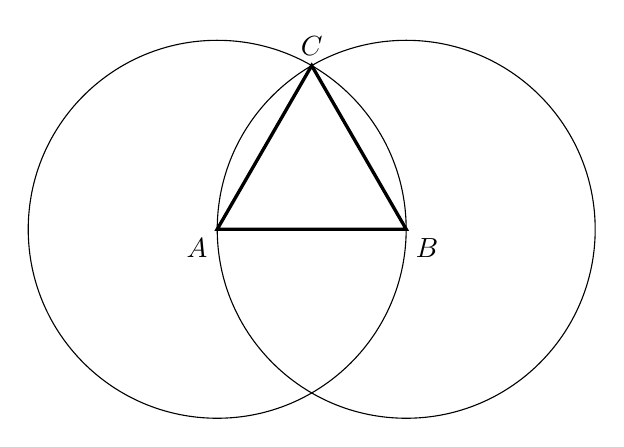
\begin{tikzpicture}[scale=1.2, line cap=round]
  \coordinate (A) at (0,0);
  \coordinate (B) at (2,0);
  \coordinate (C) at (1,{sqrt(3)});
  % Two circles, centres A and B, radius AB.
  \draw[thin] (A) circle (2);
  \draw[thin] (B) circle (2);
  % Triangle.
  \draw[very thick] (A) -- (B) -- (C) -- cycle;
  % Labels.
  \node[below left]  at (A) {$A$};
  \node[below right] at (B) {$B$};
  \node[above]       at (C) {$C$};
\end{tikzpicture}
\caption{Proposition I.1. The two circles with centres $A$ and $B$ and
common radius $AB$ meet at $C$; the triangle $ABC$ is equilateral.}
\label{fig:I.1}
\end{figure}

Let $AB$ be the given finite straight line.  With centre $A$ and
distance $AB$ describe the circle $BCD$ (Postulate 3).  With centre
$B$ and distance $BA$ describe the circle $ACE$ (Postulate 3).  From
the point $C$, where the circles cut one another, draw $CA$ and $CB$
(Postulate 1).  Since $A$ is the centre of $BCD$, $AC = AB$
(Definition I.15).  Since $B$ is the centre of $ACE$, $BC = BA$
(Definition I.15).  By Common Notion 1, $AC = BC$.  Therefore the
triangle $ABC$ is equilateral.
\dependson{I.1}{post:1}
\dependson{I.1}{post:3}
\dependson{I.1}{def:I.15}
\dependson{I.1}{cn:1}
\end{evidence}

\begin{claim}[Proposition I.2: Transfer a segment to a given point]
\label{prop:I.2}
To place at a given point (as an extremity) a straight line equal to a
given straight line.
\end{claim}
\begin{evidence}[Proof of I.2]
\label{ev:I.2}
Apply I.1 to obtain an equilateral triangle; produce its sides
(Postulate 2); describe a circle with centre at one endpoint of the
given segment cutting one of the produced sides; the cut-off equals
the given segment by Definition I.15 and Common Notion 1.
\dependson{I.2}{I.1}
\dependson{I.2}{post:1}
\dependson{I.2}{post:2}
\dependson{I.2}{post:3}
\dependson{I.2}{def:I.15}
\dependson{I.2}{cn:1}
\end{evidence}

\begin{claim}[Proposition I.3: Cut off a segment equal to a shorter]
\label{prop:I.3}
Given two unequal straight lines, to cut off from the greater a
straight line equal to the less.
\end{claim}
\begin{evidence}[Proof of I.3]
\label{ev:I.3}
Use I.2 to construct, at one extremity of the longer line, a segment
equal to the shorter.  Then by Definition I.15 the desired cut-off is
obtained.
\dependson{I.3}{I.2}
\dependson{I.3}{def:I.15}
\end{evidence}

\begin{claim}[Proposition I.4: SAS congruence]
\label{prop:I.4}
If two triangles have two sides equal to two sides respectively, and
have the angles contained by the equal straight lines equal, then they
will also have the base equal to the base, the triangle will be equal
to the triangle, and the remaining angles will be equal to the
remaining angles respectively.
\end{claim}
\begin{evidence}[Proof of I.4]
\label{ev:I.4}
Superpose one triangle on the other; corresponding sides and angles
coincide; by Common Notion 4 the figures are equal.
\dependson{I.4}{cn:4}
\end{evidence}

\begin{claim}[Proposition I.5: Pons asinorum]
\label{prop:I.5}
In isosceles triangles the angles at the base are equal to one
another; and if the equal straight lines be produced further, the
angles under the base will be equal to one another.
\end{claim}
\begin{evidence}[Proof of I.5]
\label{ev:I.5}
% [flatten-tex.py] MISSING: figures/fig-i-5
% fig-i-5.tex — I.5: pons asinorum (base angles of an isoceles triangle).
\begin{figure}[H]
\centering
\begin{tikzpicture}[scale=1.0, line cap=round]
  \coordinate (A) at (0, 3);
  \coordinate (B) at (-1.5, 0);
  \coordinate (C) at (1.5, 0);
  % Equal sides AB and AC, extended to F and G.
  \coordinate (F) at ($(A)!2.0!(B)$);
  \coordinate (G) at ($(A)!2.0!(C)$);
  \draw[thin]      (A) -- (F);
  \draw[thin]      (A) -- (G);
  \draw[very thick] (B) -- (C);
  % Points D on BF, E on CG with BD = CE.
  \coordinate (D) at ($(B)!0.5!(F)$);
  \coordinate (E) at ($(C)!0.5!(G)$);
  \draw[very thick, dashed] (B) -- (E);
  \draw[very thick, dashed] (C) -- (D);
  % Labels.
  \node[above]      at (A) {$A$};
  \node[left]       at (B) {$B$};
  \node[right]      at (C) {$C$};
  \node[below left] at (D) {$D$};
  \node[below right] at (E) {$E$};
  \node[below left] at (F) {$F$};
  \node[below right] at (G) {$G$};
\end{tikzpicture}
\caption{Proposition I.5. With $AB = AC$ and $BD = CE$ on the extensions,
triangles $ABE$ and $ACD$ are congruent (SAS, by I.4), whence the base
angles $\angle ABC = \angle ACB$.}
\label{fig:I.5}
\end{figure}

Apply I.3 to mark equal segments on the produced sides, then I.4 to
two pairs of congruent triangles.  Common Notion 3 gives equality of
the remaining angles.
\dependson{I.5}{I.3}
\dependson{I.5}{I.4}
\dependson{I.5}{cn:3}
\end{evidence}

\begin{claim}[Proposition I.6: Converse of I.5]
\label{prop:I.6}
If in a triangle two angles are equal to one another, the sides which
subtend the equal angles will also be equal to one another.
\end{claim}
\begin{evidence}[Proof of I.6]
\label{ev:I.6}
Suppose the sides unequal; cut off (by I.3) the greater equal to the
less; by I.4 the resulting smaller triangle equals the whole, which
contradicts Common Notion 5.  Therefore the sides are equal.
\dependson{I.6}{I.3}
\dependson{I.6}{I.4}
\dependson{I.6}{cn:5}
\end{evidence}

\begin{claim}[Proposition I.7: Uniqueness of triangle on a base]
\label{prop:I.7}
Given two straight lines constructed on a straight line and meeting in
a point, there cannot be constructed on the same straight line and on
the same side of it two other straight lines meeting in another point
and equal to the former two respectively, namely each to that which
has the same extremity with it.
\end{claim}
\begin{evidence}[Proof of I.7]
\label{ev:I.7}
A double application of I.5 yields contradictory angle equalities; by
Common Notion 5 the second meeting point cannot exist.
\dependson{I.7}{I.5}
\dependson{I.7}{cn:5}
\end{evidence}

\begin{claim}[Proposition I.8: SSS congruence]
\label{prop:I.8}
If two triangles have the two sides equal to two sides respectively,
and have also the base equal to the base, they will also have the
angles equal which are contained by the equal straight lines.
\end{claim}
\begin{evidence}[Proof of I.8]
\label{ev:I.8}
Superpose and apply I.7 to rule out a non-coincident image of the
contained angle; conclude by Common Notion 4.
\dependson{I.8}{I.7}
\dependson{I.8}{cn:4}
\end{evidence}

\begin{claim}[Proposition I.9: Angle bisection]
\label{prop:I.9}
To bisect a given rectilineal angle.
\end{claim}
\begin{evidence}[Proof of I.9]
\label{ev:I.9}
Apply I.1 to construct an equilateral triangle on a chord between the
angle's sides; the line from the vertex to the equilateral's apex
bisects the angle by I.8.
\dependson{I.9}{I.1}
\dependson{I.9}{I.8}
\end{evidence}

\begin{claim}[Proposition I.10: Segment bisection]
\label{prop:I.10}
To bisect a given finite straight line.
\end{claim}
\begin{evidence}[Proof of I.10]
\label{ev:I.10}
Apply I.1 to erect an equilateral triangle on the segment; bisect the
opposite angle by I.9; the bisector meets the segment at its midpoint
by I.4.
\dependson{I.10}{I.1}
\dependson{I.10}{I.9}
\dependson{I.10}{I.4}
\end{evidence}

\begin{claim}[Proposition I.11: Perpendicular at a point]
\label{prop:I.11}
To draw a straight line at right angles to a given straight line from
a given point on it.
\end{claim}
\begin{evidence}[Proof of I.11]
\label{ev:I.11}
Apply I.3 to mark equal segments either side of the given point, then
I.1 to erect an equilateral triangle whose apex line is perpendicular
(by I.8 and Definition I.10).
\dependson{I.11}{I.1}
\dependson{I.11}{I.3}
\dependson{I.11}{I.8}
\dependson{I.11}{def:I.10}
\end{evidence}

\begin{claim}[Proposition I.12: Perpendicular from external point]
\label{prop:I.12}
To draw a perpendicular straight line to a given infinite straight
line from a given point not on it.
\end{claim}
\begin{evidence}[Proof of I.12]
\label{ev:I.12}
With centre at the external point describe a circle (Postulate 3)
cutting the given line; bisect the chord by I.10; the line from the
external point to the midpoint is perpendicular by I.8.
\dependson{I.12}{I.8}
\dependson{I.12}{I.10}
\dependson{I.12}{post:3}
\end{evidence}

\begin{claim}[Proposition I.13: Adjacent angles sum to two right angles]
\label{prop:I.13}
If a straight line set up on a straight line make angles, it will
make either two right angles or angles equal to two right angles.
\end{claim}
\begin{evidence}[Proof of I.13]
\label{ev:I.13}
Drop a perpendicular by I.11; Common Notions 1--2 sum the resulting
two right angles to the unequal-case angle sum.
\dependson{I.13}{I.11}
\dependson{I.13}{cn:1}
\dependson{I.13}{cn:2}
\dependson{I.13}{def:I.10}
\end{evidence}

\begin{claim}[Proposition I.14: Converse of I.13]
\label{prop:I.14}
If with any straight line, and at a point on it, two straight lines
not lying on the same side make the adjacent angles equal to two
right angles, the two straight lines will be in a straight line with
one another.
\end{claim}
\begin{evidence}[Proof of I.14]
\label{ev:I.14}
Suppose not; then I.13 and Common Notion 1 yield contradictory angle
sums.
\dependson{I.14}{I.13}
\dependson{I.14}{cn:1}
\end{evidence}

\begin{claim}[Proposition I.15: Vertical angles]
\label{prop:I.15}
If two straight lines cut one another, they make the vertical angles
equal to one another.
\end{claim}
\begin{evidence}[Proof of I.15]
\label{ev:I.15}
Apply I.13 twice and Common Notion 3.
\dependson{I.15}{I.13}
\dependson{I.15}{cn:3}
\end{evidence}

\begin{claim}[Proposition I.16: Exterior angle of a triangle]
\label{prop:I.16}
In any triangle, if one of the sides be produced, the exterior angle
is greater than either of the interior and opposite angles.
\end{claim}
\begin{evidence}[Proof of I.16]
\label{ev:I.16}
Bisect a side by I.10; produce a median; apply I.4 to obtain a
congruent triangle that has the interior angle as one of its parts;
Common Notion 5 closes the inequality.
\dependson{I.16}{I.4}
\dependson{I.16}{I.10}
\dependson{I.16}{cn:5}
\end{evidence}

\begin{claim}[Proposition I.17: Sum of any two angles $<$ two right angles]
\label{prop:I.17}
In any triangle two angles taken together in any manner are less than
two right angles.
\end{claim}
\begin{evidence}[Proof of I.17]
\label{ev:I.17}
Apply I.16 and I.13.
\dependson{I.17}{I.13}
\dependson{I.17}{I.16}
\end{evidence}

\begin{claim}[Proposition I.18: Greater side subtends greater angle]
\label{prop:I.18}
In any triangle the greater side subtends the greater angle.
\end{claim}
\begin{evidence}[Proof of I.18]
\label{ev:I.18}
Cut off (I.3) a segment on the greater side equal to the lesser;
apply I.5 and I.16.
\dependson{I.18}{I.3}
\dependson{I.18}{I.5}
\dependson{I.18}{I.16}
\end{evidence}

\begin{claim}[Proposition I.19: Converse of I.18]
\label{prop:I.19}
In any triangle the greater angle is subtended by the greater side.
\end{claim}
\begin{evidence}[Proof of I.19]
\label{ev:I.19}
Suppose not; by I.5 and I.18 contradiction.
\dependson{I.19}{I.5}
\dependson{I.19}{I.18}
\end{evidence}

\begin{claim}[Proposition I.20: Triangle inequality]
\label{prop:I.20}
In any triangle two sides taken together in any manner are greater
than the remaining one.
\end{claim}
\begin{evidence}[Proof of I.20]
\label{ev:I.20}
Produce one side to an isosceles configuration by I.3; apply I.5 and
I.19.
\dependson{I.20}{I.3}
\dependson{I.20}{I.5}
\dependson{I.20}{I.19}
\end{evidence}

\begin{claim}[Proposition I.21: Interior cevian inequalities]
\label{prop:I.21}
If on one of the sides of a triangle, from its extremities, there be
constructed two straight lines meeting within the triangle, the
straight lines so constructed will be less than the remaining two
sides of the triangle, but will contain a greater angle.
\end{claim}
\begin{evidence}[Proof of I.21]
\label{ev:I.21}
Two applications of I.20 and one of I.16.
\dependson{I.21}{I.16}
\dependson{I.21}{I.20}
\end{evidence}

\begin{claim}[Proposition I.22: Triangle from three given segments]
\label{prop:I.22}
Out of three straight lines, which are equal to three given straight
lines, to construct a triangle: thus it is necessary that two of the
straight lines taken together in any manner should be greater than the
remaining one.
\end{claim}
\begin{evidence}[Proof of I.22]
\label{ev:I.22}
Apply I.20 (the necessity), then I.3 and Postulate 3 (the
construction).
\dependson{I.22}{I.3}
\dependson{I.22}{I.20}
\dependson{I.22}{post:3}
\end{evidence}

\begin{claim}[Proposition I.23: Reproduce a given angle]
\label{prop:I.23}
On a given straight line and at a point on it to construct a
rectilineal angle equal to a given rectilineal angle.
\end{claim}
\begin{evidence}[Proof of I.23]
\label{ev:I.23}
Cut equal segments by I.3, construct the matching triangle by I.22,
apply I.8.
\dependson{I.23}{I.3}
\dependson{I.23}{I.8}
\dependson{I.23}{I.22}
\end{evidence}

\begin{claim}[Proposition I.24: Hinge inequality]
\label{prop:I.24}
If two triangles have the two sides equal to two sides respectively,
but have the one of the angles contained by the equal straight lines
greater than the other, they will also have the base greater than the
base.
\end{claim}
\begin{evidence}[Proof of I.24]
\label{ev:I.24}
Apply I.23, I.4, I.5, and I.19.
\dependson{I.24}{I.4}
\dependson{I.24}{I.5}
\dependson{I.24}{I.19}
\dependson{I.24}{I.23}
\end{evidence}

\begin{claim}[Proposition I.25: Converse of I.24]
\label{prop:I.25}
If two triangles have the two sides equal to two sides respectively,
but have the one base greater than the other, they will also have the
one angle contained by the equal straight lines greater than the
other.
\end{claim}
\begin{evidence}[Proof of I.25]
\label{ev:I.25}
Suppose not and use I.4, I.24.
\dependson{I.25}{I.4}
\dependson{I.25}{I.24}
\end{evidence}

\begin{claim}[Proposition I.26: ASA / AAS congruence]
\label{prop:I.26}
If two triangles have the two angles equal to two angles respectively,
and one side equal to one side, namely either the side adjoining the
equal angles or that subtending one of the equal angles, they will
also have the remaining sides equal to the remaining sides and the
remaining angle equal to the remaining angle.
\end{claim}
\begin{evidence}[Proof of I.26]
\label{ev:I.26}
Apply I.4 to the congruent angle--side--angle case; for the AAS case
combine I.4 with I.16.
\dependson{I.26}{I.4}
\dependson{I.26}{I.16}
\end{evidence}

\begin{claim}[Proposition I.27: Alternate angles imply parallels]
\label{prop:I.27}
If a straight line falling on two straight lines make the alternate
angles equal to one another, the straight lines will be parallel to
one another.
\end{claim}
\begin{evidence}[Proof of I.27]
\label{ev:I.27}
Suppose the lines meet; I.16 gives a contradiction.  By Definition
I.23 they are parallel.
\dependson{I.27}{I.16}
\dependson{I.27}{def:I.23}
\end{evidence}

\begin{claim}[Proposition I.28: Corresponding angles imply parallels]
\label{prop:I.28}
If a straight line falling on two straight lines make the exterior
angle equal to the interior and opposite angle on the same side, or
the interior angles on the same side equal to two right angles, the
straight lines will be parallel to one another.
\end{claim}
\begin{evidence}[Proof of I.28]
\label{ev:I.28}
Reduce to I.27 via I.13 and I.15.
\dependson{I.28}{I.13}
\dependson{I.28}{I.15}
\dependson{I.28}{I.27}
\end{evidence}

\begin{claim}[Proposition I.29: Properties of parallels (uses Postulate 5)]
\label{prop:I.29}
A straight line falling on parallel straight lines makes the alternate
angles equal to one another, the exterior angle equal to the interior
and opposite angle, and the interior angles on the same side equal to
two right angles.
\end{claim}
\begin{evidence}[Proof of I.29]
\label{ev:I.29}
The first use of Postulate 5: any contrary supposition contradicts the
parallel postulate via I.13.
\dependson{I.29}{I.13}
\dependson{I.29}{post:5}
\end{evidence}

\begin{claim}[Proposition I.30: Transitivity of parallelism]
\label{prop:I.30}
Straight lines parallel to the same straight line are also parallel
to one another.
\end{claim}
\begin{evidence}[Proof of I.30]
\label{ev:I.30}
Two applications of I.29 and Common Notion 1.
\dependson{I.30}{I.29}
\dependson{I.30}{cn:1}
\end{evidence}

\begin{claim}[Proposition I.31: Construct a parallel through a point]
\label{prop:I.31}
Through a given point to draw a straight line parallel to a given
straight line.
\end{claim}
\begin{evidence}[Proof of I.31]
\label{ev:I.31}
Apply I.23 to reproduce the alternate angle at the given point and
I.27 to conclude parallelism.
\dependson{I.31}{I.23}
\dependson{I.31}{I.27}
\end{evidence}

\begin{claim}[Proposition I.32: Triangle angle sum]
\label{prop:I.32}
In any triangle, if one of the sides be produced, the exterior angle
is equal to the two interior and opposite angles, and the three
interior angles of the triangle are equal to two right angles.
\end{claim}
\begin{evidence}[Proof of I.32]
% [flatten-tex.py] MISSING: figures/fig-i-32
% fig-i-32.tex — I.32: triangle angle sum (parallel through apex).
\begin{figure}[H]
\centering
\begin{tikzpicture}[scale=1.2, line cap=round]
  \coordinate (A) at (-1.5, 0);
  \coordinate (B) at (2.0, 0);
  \coordinate (C) at (0.5, 2.4);
  \coordinate (D) at ($(C)!-1.4!(A)$); % line through C parallel to AB, on left
  \coordinate (E) at ($(C)!-1.4!(B)$); % line through C parallel to AB, on right
  % Triangle.
  \draw[very thick] (A) -- (B) -- (C) -- cycle;
  % Parallel through C, drawn long.
  \draw[thin] ($(C)!-0.7!(B)$) -- ($(C)!1.5!(B)$);
  % Side AB extended beyond B to F to expose exterior angle.
  \coordinate (F) at ($(A)!1.4!(B)$);
  \draw[thin] (B) -- (F);
  % Labels.
  \node[below left]  at (A) {$A$};
  \node[below right] at (B) {$B$};
  \node[above]       at (C) {$C$};
  \node[below right] at (F) {$F$};
  \node[above left]  at ($(C)!-0.7!(B)$) {$D$};
  \node[above right] at ($(C)!1.5!(B)$) {$E$};
\end{tikzpicture}
\caption{Proposition I.32. Drawing $DE$ through $C$ parallel to $AB$
makes $\angle DCA = \angle CAB$ (alternate, I.29) and $\angle ECB =
\angle ABC$ (alternate, I.29); the straight angle at $C$ then sums
the three interior angles of $\triangle ABC$ to two right angles.}
\label{fig:I.32}
\end{figure}

\label{ev:I.32}
Apply I.31 to draw a parallel through the apex; apply I.29 twice and
Common Notion 2.
\dependson{I.32}{I.29}
\dependson{I.32}{I.31}
\dependson{I.32}{cn:2}
\end{evidence}

\begin{claim}[Proposition I.33: Connecting equal-and-parallel pairs]
\label{prop:I.33}
The straight lines joining equal and parallel straight lines (at the
extremities which are in the same directions) are themselves equal
and parallel.
\end{claim}
\begin{evidence}[Proof of I.33]
\label{ev:I.33}
Apply I.4 to the resulting two triangles and I.29 + I.27 for
parallelism.
\dependson{I.33}{I.4}
\dependson{I.33}{I.27}
\dependson{I.33}{I.29}
\end{evidence}

\begin{claim}[Proposition I.34: Properties of parallelograms]
\label{prop:I.34}
In parallelogrammic areas the opposite sides and angles are equal to
one another, and the diameter bisects the areas.
\end{claim}
\begin{evidence}[Proof of I.34]
\label{ev:I.34}
Apply I.29 and I.26 to the two triangles cut by the diameter, then
Common Notion 2.
\dependson{I.34}{I.26}
\dependson{I.34}{I.29}
\dependson{I.34}{cn:2}
\end{evidence}

\begin{claim}[Proposition I.35: Parallelograms with same base \& between same parallels]
\label{prop:I.35}
Parallelograms which are on the same base and in the same parallels
are equal to one another.
\end{claim}
\begin{evidence}[Proof of I.35]
\label{ev:I.35}
Apply I.34 and I.4 to congruent triangles; conclude by Common Notions
2--3.
\dependson{I.35}{I.4}
\dependson{I.35}{I.34}
\dependson{I.35}{cn:2}
\dependson{I.35}{cn:3}
\end{evidence}

\begin{claim}[Proposition I.36: Parallelograms with equal bases]
\label{prop:I.36}
Parallelograms which are on equal bases and in the same parallels are
equal to one another.
\end{claim}
\begin{evidence}[Proof of I.36]
\label{ev:I.36}
Translate one parallelogram via I.33 to share a base with the other,
then apply I.35.
\dependson{I.36}{I.33}
\dependson{I.36}{I.35}
\end{evidence}

\begin{claim}[Proposition I.37: Triangles with same base \& parallels]
\label{prop:I.37}
Triangles which are on the same base and in the same parallels are
equal to one another.
\end{claim}
\begin{evidence}[Proof of I.37]
\label{ev:I.37}
Complete each triangle to a parallelogram via I.31, then apply I.34
and I.35.
\dependson{I.37}{I.31}
\dependson{I.37}{I.34}
\dependson{I.37}{I.35}
\end{evidence}

\begin{claim}[Proposition I.38: Triangles with equal bases]
\label{prop:I.38}
Triangles which are on equal bases and in the same parallels are
equal to one another.
\end{claim}
\begin{evidence}[Proof of I.38]
\label{ev:I.38}
Same construction as I.37 with I.36 in place of I.35.
\dependson{I.38}{I.31}
\dependson{I.38}{I.34}
\dependson{I.38}{I.36}
\end{evidence}

\begin{claim}[Proposition I.39: Equal triangles on same base $\Rightarrow$ same parallels]
\label{prop:I.39}
Equal triangles which are on the same base and on the same side are
also in the same parallels.
\end{claim}
\begin{evidence}[Proof of I.39]
\label{ev:I.39}
Apply I.31 to draw a parallel; I.37 forces the second vertex onto it.
\dependson{I.39}{I.31}
\dependson{I.39}{I.37}
\end{evidence}

\begin{claim}[Proposition I.40: Equal triangles on equal bases]
\label{prop:I.40}
Equal triangles which are on equal bases and on the same side are
also in the same parallels.
\end{claim}
\begin{evidence}[Proof of I.40]
\label{ev:I.40}
Same approach as I.39 with I.38 in place of I.37.
\dependson{I.40}{I.31}
\dependson{I.40}{I.38}
\end{evidence}

\begin{claim}[Proposition I.41: Parallelogram is double a triangle]
\label{prop:I.41}
If a parallelogram have the same base with a triangle and be in the
same parallels, the parallelogram is double of the triangle.
\end{claim}
\begin{evidence}[Proof of I.41]
\label{ev:I.41}
Apply I.34 and I.37; double via Common Notion 2.
\dependson{I.41}{I.34}
\dependson{I.41}{I.37}
\dependson{I.41}{cn:2}
\end{evidence}

\begin{claim}[Proposition I.42: Construct a parallelogram equal in area to a triangle]
\label{prop:I.42}
To construct, in a given rectilineal angle, a parallelogram equal to
a given triangle.
\end{claim}
\begin{evidence}[Proof of I.42]
\label{ev:I.42}
Bisect a side by I.10; apply I.23 to set the angle; apply I.31 and
I.41.
\dependson{I.42}{I.10}
\dependson{I.42}{I.23}
\dependson{I.42}{I.31}
\dependson{I.42}{I.41}
\end{evidence}

\begin{claim}[Proposition I.43: Complements of a parallelogram]
\label{prop:I.43}
In any parallelogram the complements of the parallelograms about the
diameter are equal to one another.
\end{claim}
\begin{evidence}[Proof of I.43]
\label{ev:I.43}
Apply I.34 to the bisecting diameter and Common Notions 2--3.
\dependson{I.43}{I.34}
\dependson{I.43}{cn:2}
\dependson{I.43}{cn:3}
\end{evidence}

\begin{claim}[Proposition I.44: Apply a parallelogram to a segment equal to a triangle]
\label{prop:I.44}
To a given straight line to apply, in a given rectilineal angle, a
parallelogram equal to a given triangle.
\end{claim}
\begin{evidence}[Proof of I.44]
\label{ev:I.44}
Apply I.42 and I.43 in sequence.
\dependson{I.44}{I.42}
\dependson{I.44}{I.43}
\end{evidence}

\begin{claim}[Proposition I.45: Apply a parallelogram equal to a rectilineal figure]
\label{prop:I.45}
To construct, in a given rectilineal angle, a parallelogram equal to
a given rectilineal figure.
\end{claim}
\begin{evidence}[Proof of I.45]
\label{ev:I.45}
Triangulate the figure; sum the parallelograms by repeated I.44 and
Common Notion 2.
\dependson{I.45}{I.44}
\dependson{I.45}{cn:2}
\end{evidence}

\begin{claim}[Proposition I.46: Construct a square on a segment]
\label{prop:I.46}
On a given straight line to describe a square.
\end{claim}
\begin{evidence}[Proof of I.46]
\label{ev:I.46}
Apply I.11 to erect perpendiculars; use I.3 to cut off equal segments;
use I.31 and I.29 to close the square; verify right angles via I.34.
\dependson{I.46}{I.3}
\dependson{I.46}{I.11}
\dependson{I.46}{I.29}
\dependson{I.46}{I.31}
\dependson{I.46}{I.34}
\end{evidence}

\begin{claim}[Proposition I.47: Pythagoras' theorem]
\label{prop:I.47}
In right-angled triangles the square on the side subtending the right
angle is equal to the squares on the sides containing the right angle.
\end{claim}
\begin{evidence}[Proof of I.47]
% [flatten-tex.py] MISSING: figures/fig-i-47
% fig-i-47.tex — I.47: Pythagoras (square decomposition).
\begin{figure}[H]
\centering
\begin{tikzpicture}[scale=0.55, line cap=round, line join=round]
  % Right triangle vertices: right angle at A.
  \coordinate (A) at (0, 0);
  \coordinate (B) at (3, 0); % horizontal leg
  \coordinate (C) at (0, 4); % vertical leg
  % Hypotenuse BC.
  % Square on AB (below): A, B, B', A'
  \coordinate (Ap) at (0, -3);
  \coordinate (Bp) at (3, -3);
  % Square on AC (left): A, C, C', A''
  \coordinate (App) at (-4, 0);
  \coordinate (Cp)  at (-4, 4);
  % Square on BC (outward): B, C, C'', B''
  % Outward direction = rotate (B-C) by -90.
  \coordinate (Bpp) at ($(B)!1!-90:(C)$);
  \coordinate (Cpp) at ($(C)!1!90:(B)$);
  % Triangle.
  \draw[very thick] (A) -- (B) -- (C) -- cycle;
  % Three squares.
  \draw[thick, fill=gray!10] (A)   -- (B)   -- (Bp)  -- (Ap)  -- cycle;
  \draw[thick, fill=gray!10] (A)   -- (C)   -- (Cp)  -- (App) -- cycle;
  \draw[thick, fill=gray!20] (B)   -- (C)   -- (Cpp) -- (Bpp) -- cycle;
  % Altitude from A to BC, foot at H, extended to meet square on BC.
  \coordinate (H) at ($(B)!(A)!(C)$);
  \coordinate (Hext) at ($(H)!1!-90:(B)$);
  \draw[thin, dashed] (A) -- (Hext);
  % Labels.
  \node[below right]      at (A) {$A$};
  \node[below]            at (B) {$B$};
  \node[left]             at (C) {$C$};
  \node[left]             at ($(A)!0.5!(App)$) {square on $AC$};
  \node                   at ($(A)!0.5!(Bp)+(0.5,-1.5)$) {square on $AB$};
  \node                   at ($(B)!0.5!(Cpp)+(1.7,0.7)$) {square on $BC$};
\end{tikzpicture}
\caption{Proposition I.47. The square on the hypotenuse $BC$ is
partitioned by the altitude $AH$ extended into two rectangles, each
equal (by I.41 + I.46) to a square on a leg; thus $BC^2 = AB^2 + AC^2$.}
\label{fig:I.47}
\end{figure}

\label{ev:I.47}
Erect squares on each side via I.46; using I.14, I.31 and I.41 show
each part-square equals a corresponding parallelogram cut off the
hypotenuse-square by the perpendicular from the right angle; sum via
Common Notion 2.
\dependson{I.47}{I.4}
\dependson{I.47}{I.14}
\dependson{I.47}{I.31}
\dependson{I.47}{I.41}
\dependson{I.47}{I.46}
\dependson{I.47}{cn:2}
\supports{I.47}{I.48}
\end{evidence}

\begin{claim}[Proposition I.48: Converse of Pythagoras]
\label{prop:I.48}
If in a triangle the square on one of the sides be equal to the
squares on the remaining two sides of the triangle, the angle
contained by the remaining two sides of the triangle is right.
\end{claim}
\begin{evidence}[Proof of I.48]
\label{ev:I.48}
Construct a right triangle with the same two legs by I.11; apply
I.47, I.8, and Common Notion 1.
\dependson{I.48}{I.8}
\dependson{I.48}{I.11}
\dependson{I.48}{I.47}
\dependson{I.48}{cn:1}
\end{evidence}
% [flatten-tex.py] end: books/book01.tex
% [flatten-tex.py] inlined: books/book02.tex
% book02.tex --- Book II of Euclid's Elements: Geometric Algebra.
%
% The propositions of Book II are the classical identities of "geometric
% algebra" --- distributivity, the binomial squares, and the law of
% cosines in its purely-geometric form (II.12, II.13). All proofs go
% through the gnomon construction (Definition II.2) and rely on Book I,
% chiefly I.34, I.41, I.43, I.46, and I.47.
%
% Statement wording follows Heath (1908); proof prose mirrors Heath's
% density --- explicit construction steps with inline lemma citations.

\section{Book II --- Geometric Algebra}
\label{sec:book-II}

\begin{claim}[Proposition II.1: Distributivity of multiplication]
\label{prop:II.1}
If there be two straight lines, and one of them be cut into any
number of segments whatever, the rectangle contained by the two
straight lines is equal to the rectangles contained by the
uncut straight line and each of the segments.
\end{claim}
\begin{evidence}[Proof of II.1]
\label{ev:II.1}
Let $A$ and $BC$ be the two straight lines, and let $BC$ be cut at
random at the points $D$, $E$.  Construct the rectangle contained by
$A$ and $BC$ as follows.  From $B$ draw $BF$ at right angles to $BC$
(I.11) with $BF$ equal to $A$.  Through $F$ draw $FG$ parallel to $BC$
(I.31), and through $C$, $D$, $E$ in turn draw $CH$, $DK$, $EL$
parallel to $BF$ (I.31).  Then the rectangle $BH$ on the lines $A$,
$BC$ is divided by the parallels $DK$, $EL$ into the three rectangles
$BK$ on $A$, $BD$; $DL$ on $A$, $DE$; and $EH$ on $A$, $EC$
(Definition II.1).  By Common Notion 2, the whole rectangle equals
the sum of these parts: $A \cdot BC = A\cdot BD + A\cdot DE +
A\cdot EC$.  The argument generalises to any number of cuts on $BC$.
\dependson{II.1}{I.11}
\dependson{II.1}{I.31}
\dependson{II.1}{I.34}
\dependson{II.1}{cn:2}
\dependson{II.1}{def:II.1}
\end{evidence}

\begin{claim}[Proposition II.2: Whole equals sum of rectangles on parts]
\label{prop:II.2}
If a straight line be cut at random, the rectangle contained by the
whole and both of the segments is equal to the square on the whole.
\end{claim}
\begin{evidence}[Proof of II.2]
\label{ev:II.2}
Let the straight line $AB$ be cut at random at the point $C$.
Describe on $AB$ the square $ADEB$ (I.46), and through $C$ draw
$CF$ parallel to either $AD$ or $BE$ (I.31), so that $CF$ meets $DE$
at $F$.  The square $ADEB$ is thereby divided into two rectangles:
$ADFC$ contained by $AD$ and $AC$ (and since $AD = AB$, this rectangle
is contained by $AB$ and $AC$, by Definition II.1), and $CFEB$
contained by $CF$ and $CB$ (again, $CF = AB$, so this rectangle is
contained by $AB$ and $CB$).  Their sum (Common Notion 2) is the
whole square $ADEB$, which is the square on $AB$.  Therefore the
rectangle on $AB$ and $AC$ together with the rectangle on $AB$ and
$CB$ equals the square on $AB$.
\dependson{II.2}{I.31}
\dependson{II.2}{I.34}
\dependson{II.2}{I.46}
\dependson{II.2}{cn:2}
\dependson{II.2}{def:II.1}
\end{evidence}

\begin{claim}[Proposition II.3: Rectangle on a part equals rect on parts plus square]
\label{prop:II.3}
If a straight line be cut at random, the rectangle contained by the
whole and one of the segments is equal to the rectangle contained by
the segments and the square on the aforesaid segment.
\end{claim}
\begin{evidence}[Proof of II.3]
\label{ev:II.3}
Let $AB$ be cut at $C$; consider the rectangle on $AB$, $AC$.  By
Proposition II.1, taking $AB$ as the uncut line and the two segments
$AC$, $CB$ of $AB$ itself as the cut line, the rectangle on $AB$ and
$AC$ equals the rectangle on $AC$ and $AC$ together with the
rectangle on $AB$ and $CB$ --- but the rectangle on $AC$ and $AC$ is
the square on $AC$ by Definition II.1.  Re-expressing the rectangle
on $AB$ and $CB$ via II.1 again as the rectangle on $AC$, $CB$ plus
the rectangle on $CB$, $CB$ (which is the square on $CB$, again by
Definition II.1) and combining, we obtain:
the rectangle on $AB$ and $AC$ equals the rectangle on $AC$ and
$CB$ plus the square on $AC$.  By Common Notion 2 the equality is
preserved when rearranged.
\dependson{II.3}{II.1}
\dependson{II.3}{def:II.1}
\dependson{II.3}{cn:2}
\end{evidence}

\begin{claim}[Proposition II.4: Square of a sum is sum of squares plus twice rectangle]
\label{prop:II.4}
If a straight line be cut at random, the square on the whole is equal
to the squares on the segments and twice the rectangle contained by
the segments.
\end{claim}
\begin{evidence}[Proof of II.4]
\label{ev:II.4}
% [flatten-tex.py] MISSING: figures/fig-ii-4
% fig-ii-4.tex — II.4: binomial square (a+b)^2 = a^2 + 2ab + b^2.
\begin{figure}[H]
\centering
\begin{tikzpicture}[scale=1.0, line cap=round, line join=round]
  \def\a{2.4}
  \def\b{1.4}
  \coordinate (A) at (0, 0);
  \coordinate (B) at ({\a+\b}, 0);
  \coordinate (D) at (0, {\a+\b});
  \coordinate (E) at ({\a+\b}, {\a+\b});
  \coordinate (C) at (\a, 0);
  \coordinate (G) at (\a, \a);
  \coordinate (F) at (\a, {\a+\b});
  \coordinate (H) at (0, \a);
  \coordinate (K) at ({\a+\b}, \a);
  % Outer square ADEB.
  \draw[very thick] (A) -- (B) -- (E) -- (D) -- cycle;
  % Diagonal BD.
  \draw[thin, dashed] (B) -- (D);
  % Internal partition: CF parallel to AD, HK parallel to AB.
  \draw[thick] (C) -- (F);
  \draw[thick] (H) -- (K);
  % Shaded squares: HDFG (top-left, side a) and CBKG (bottom-right, side b).
  \fill[gray!10] (H) -- (D) -- (F) -- (G) -- cycle;
  \fill[gray!25] (C) -- (B) -- (K) -- (G) -- cycle;
  % Re-draw lines on top so shading doesn't hide them.
  \draw[very thick] (A) -- (B) -- (E) -- (D) -- cycle;
  \draw[thick] (C) -- (F);
  \draw[thick] (H) -- (K);
  \draw[thin, dashed] (B) -- (D);
  % Labels.
  \node[below left]  at (A) {$A$};
  \node[below]       at (C) {$C$};
  \node[below right] at (B) {$B$};
  \node[above left]  at (D) {$D$};
  \node[above]       at (F) {$F$};
  \node[above right] at (E) {$E$};
  \node[left]        at (H) {$H$};
  \node[right]       at (K) {$K$};
  \node              at (G) {$G$};
  % Side annotations.
  \node[below] at ($(A)!0.5!(C)$) {$a$};
  \node[below] at ($(C)!0.5!(B)$) {$b$};
\end{tikzpicture}
\caption{Proposition II.4. The square $ADEB$ on $AB = a+b$ is
decomposed by the parallels $CF \parallel AD$ and $HK \parallel AB$
into the square $HDFG$ on $AC = a$, the square $CBKG$ on $CB = b$, and
two equal rectangles $AGHD$ and $GFBK$ (by I.43), each equal to
$a \cdot b$.}
\label{fig:II.4}
\end{figure}

Let the straight line $AB$ be cut at random at $C$.  Describe on $AB$
the square $ADEB$ (I.46), and draw the diagonal $BD$.  Through $C$
draw $CGF$ parallel to either $AD$ or $BE$ (I.31), meeting $BD$ at
$G$ and $DE$ at $F$.  Through $G$ draw $HK$ parallel to either $AB$
or $DE$ (I.31), meeting $AD$ at $H$ and $BE$ at $K$.

Since $CF$ is parallel to $AD$ and $BD$ falls on them, the exterior
angle $\angle BGC$ equals the interior and opposite $\angle BDA$
(I.29).  But $\angle BDA = \angle DBA$ since $BA = AD$ (I.5 applied
to the isoceles right triangle inside the square).  Hence
$\angle BGC = \angle GBC$, so $BC = CG$ (I.6), and therefore $CBKG$
is equilateral.  Since it has a right angle at $B$, it is a square
on $CB$ (Definition I.22).  By the same reasoning $HDFG$ is the
square on $HD = AC$.

The complements $AGHD$ and $GFBK$ in the square $ADEB$ are equal
rectangles by I.43; each is contained by $AC$ and $CB$ (since
$AH = AC$, $HG = CB$, etc.), so each is the rectangle on $AC$, $CB$.
The four pieces sum to the whole (Common Notion 2):
\[
    AB^2 \;=\; AC^2 + CB^2 + 2\cdot(AC\cdot CB),
\]
which is $(a+b)^2 = a^2 + 2ab + b^2$ in geometric form.
\dependson{II.4}{I.5}
\dependson{II.4}{I.6}
\dependson{II.4}{I.29}
\dependson{II.4}{I.31}
\dependson{II.4}{I.34}
\dependson{II.4}{I.43}
\dependson{II.4}{I.46}
\dependson{II.4}{cn:2}
\dependson{II.4}{def:I.22}
\dependson{II.4}{def:II.1}
\dependson{II.4}{def:II.2}
\end{evidence}

\begin{claim}[Proposition II.5: Rectangle on unequal parts plus square on difference]
\label{prop:II.5}
If a straight line be cut into equal and unequal segments, the
rectangle contained by the unequal segments of the whole together with
the square on the straight line between the points of section is equal
to the square on the half.
\end{claim}
\begin{evidence}[Proof of II.5]
\label{ev:II.5}
Let $AB$ be bisected at $C$ (I.10) and cut unequally at $D$.
Describe on $CB$ the square $CEFB$ (I.46), join $BE$, and through $D$
draw $DG$ parallel to $CE$ or $BF$ (I.31), meeting $BE$ at $H$ and
$EF$ at $G$.  Through $H$ draw $KM$ parallel to $AB$ or $EF$ (I.31),
meeting $CE$ at $L$ and $BF$ at $M$.  Through $A$ draw $AK$ parallel
to $CL$ or $BM$ (I.31), meeting $KM$ extended at $K$.

The complement $CH$ equals the complement $HF$ in the square $CEFB$
(I.43).  Add to each the square $DM$; then the rectangle $CDHL$ plus
the square $LHMG$ equals the rectangle $DBFG$ plus the same square.
But $CDHL$ together with rectangle $AC$-equivalent piece $AKLC$
(which equals $CDHL$ since $AC = CB$ and the lines are parallel)
fills the gnomon $NOP$, plus the square $LHMG$ on $CD$, equals the
square $CEFB$ on $CB$.  Thus the rectangle $AD\cdot DB$ together
with the square on $CD$ equals the square on $CB$.
\dependson{II.5}{I.10}
\dependson{II.5}{I.31}
\dependson{II.5}{I.34}
\dependson{II.5}{I.36}
\dependson{II.5}{I.43}
\dependson{II.5}{I.46}
\dependson{II.5}{cn:2}
\dependson{II.5}{def:II.1}
\dependson{II.5}{def:II.2}
\end{evidence}

\begin{claim}[Proposition II.6: Rectangle on bisected-and-produced line]
\label{prop:II.6}
If a straight line be bisected and a straight line be added to it in
a straight line, the rectangle contained by the whole with the added
straight line and the added straight line, together with the square
on the half, is equal to the square on the straight line made up of
the half and the added straight line.
\end{claim}
\begin{evidence}[Proof of II.6]
\label{ev:II.6}
Let $AB$ be bisected at $C$ (I.10) and produced to $D$, so that $CD$
is the half plus the added segment $BD$.  Describe on $CD$ the
square $CEFD$ (I.46), join $DE$, and through $B$ draw $BG$ parallel
to $CE$ or $DF$ (I.31), meeting $DE$ at $H$ and $EF$ at $G$.
Through $H$ draw $KM$ parallel to $AD$ or $EF$ (I.31), and through
$A$ draw $AK$ parallel to $CL$ or $DM$ (I.31).

As in II.5, the complement $CH$ equals the complement $HF$ (I.43).
Adding the square $LHMG$ (which is the square on $BC = CB$) to both
of $CH + AL$ (the rectangle on $AD$, $DB$) shows that the rectangle
$AD\cdot DB$ together with the square on $CB$ equals the gnomon plus
the small square, which is the square $CEFD$ on $CD$.  Hence
$AD\cdot DB + CB^2 = CD^2$ as required.
\dependson{II.6}{I.10}
\dependson{II.6}{I.31}
\dependson{II.6}{I.34}
\dependson{II.6}{I.43}
\dependson{II.6}{I.46}
\dependson{II.6}{II.5}
\dependson{II.6}{cn:2}
\dependson{II.6}{def:II.1}
\dependson{II.6}{def:II.2}
\end{evidence}

\begin{claim}[Proposition II.7: Squares on whole and segment equal twice rect plus square on remainder]
\label{prop:II.7}
If a straight line be cut at random, the square on the whole and that
on one of the segments both together are equal to twice the rectangle
contained by the whole and the said segment together with the square
on the remaining segment.
\end{claim}
\begin{evidence}[Proof of II.7]
\label{ev:II.7}
Let $AB$ be cut at $C$.  Describe on $AB$ the square $ADEB$ (I.46),
and through $C$ draw $CF$ parallel to $AD$ or $BE$ (I.31), meeting
$DE$ at $F$.  On $CB$ as side construct the square $CBKG$ inside
$ADEB$ (a copy of II.4's construction), with $HK$ parallel to $AB$.

By II.4 the square $ADEB$ on $AB$ equals the square on $AC$ plus the
square on $CB$ plus twice the rectangle $AC \cdot CB$.  Add the
square on $CB$ to both sides of this identity (Common Notion 2):
\[
    AB^2 + CB^2 \;=\; AC^2 + 2\cdot CB^2 + 2\cdot(AC\cdot CB).
\]
But $2\cdot CB^2 + 2\cdot(AC\cdot CB) = 2\cdot CB(CB + AC) =
2\cdot CB \cdot AB$ (Definition II.1; II.1).  Hence
$AB^2 + CB^2 = 2\cdot(AB\cdot CB) + AC^2$, as required.
\dependson{II.7}{II.1}
\dependson{II.7}{II.4}
\dependson{II.7}{cn:2}
\dependson{II.7}{cn:3}
\dependson{II.7}{def:II.1}
\dependson{II.7}{def:II.2}
\end{evidence}

\begin{claim}[Proposition II.8: Four-times rectangle plus square on remainder equals square on sum]
\label{prop:II.8}
If a straight line be cut at random, four times the rectangle
contained by the whole and one of the segments together with the
square on the remaining segment is equal to the square described on
the whole and the aforesaid segment as on one straight line.
\end{claim}
\begin{evidence}[Proof of II.8]
\label{ev:II.8}
Let $AB$ be cut at $C$, and produce $AB$ to $D$ so that $BD = BC$.
Then $AD = AB + BC$ and $AD$ is cut at $B$ into the segments $AB$
and $BD = BC$.  Apply II.4 to the line $AD$ cut at $B$: the square
on $AD$ equals the squares on $AB$ and $BD$ together with twice the
rectangle on $AB$, $BD$.  Since $BD = BC$, this becomes:
\[
    AD^2 \;=\; AB^2 + BC^2 + 2\cdot(AB\cdot BC).
\]
Apply II.4 again to $AB$ cut at $C$, namely $AB^2 = AC^2 + CB^2 +
2\cdot(AC\cdot CB)$, and substitute.  Combining (Common Notion 2)
and re-arranging (Common Notion 3) to isolate $4\cdot(AB\cdot BC)$
on the right side yields:
\[
    AD^2 \;=\; 4\cdot(AB\cdot BC) + AC^2,
\]
which is $(a+b)^2 = 4ab + (a-b)^2$ in the form Euclid states it.
\dependson{II.8}{II.1}
\dependson{II.8}{II.4}
\dependson{II.8}{cn:2}
\dependson{II.8}{cn:3}
\dependson{II.8}{def:II.1}
\dependson{II.8}{def:II.2}
\end{evidence}

\begin{claim}[Proposition II.9: Squares on unequal segments equal double of two squares]
\label{prop:II.9}
If a straight line be cut into equal and unequal segments, the
squares on the unequal segments of the whole are double of the square
on the half and of the square on the straight line between the points
of section.
\end{claim}
\begin{evidence}[Proof of II.9]
\label{ev:II.9}
Let $AB$ be bisected at $C$ (I.10) and cut unequally at $D$.  At $C$
draw $CE$ at right angles to $AB$ (I.11), with $CE = AC = CB$.  Join
$EA$ and $EB$; through $D$ draw $DF$ parallel to $CE$ (I.31), meeting
$EB$ at $F$; through $F$ draw $FG$ parallel to $AB$ (I.31), meeting
$CE$ at $G$.  Join $AF$.

Since $\angle ECA$ is a right angle and $CA = CE$, the triangle
$ACE$ is right-isoceles, and $\angle CAE = \angle AEC = $ half a right
angle (I.5; I.32).  Similarly $\angle CBE = \angle CEB = $ half a
right angle.  Hence $\angle AEB$ is a right angle (Common Notion 2),
and triangle $AEB$ is right-angled at $E$.  By I.47:
\[
    AB^2 \;=\; AE^2 + EB^2.
\]
Now $AE^2 = AC^2 + CE^2 = 2\cdot AC^2$ (I.47 in $\triangle ACE$,
plus $CE = AC$).  Similarly inside the right triangles formed by the
perpendicular $DF$ at $D$ on $AB$, I.47 plus the fact that
$DF = DE$ (which one shows from the parallel construction)
yields, after Common Notions 2 and 3:
\[
    AD^2 + DB^2 \;=\; 2\cdot AC^2 + 2\cdot CD^2.
\]
\dependson{II.9}{I.5}
\dependson{II.9}{I.10}
\dependson{II.9}{I.11}
\dependson{II.9}{I.29}
\dependson{II.9}{I.31}
\dependson{II.9}{I.32}
\dependson{II.9}{I.34}
\dependson{II.9}{I.47}
\dependson{II.9}{cn:2}
\dependson{II.9}{cn:3}
\end{evidence}

\begin{claim}[Proposition II.10: Squares on whole-with-addition and addition equal double of two squares]
\label{prop:II.10}
If a straight line be bisected and a straight line be added to it in
a straight line, the square on the whole with the added straight line
and the square on the added straight line both together are double of
the square on the half and of the square described on the straight
line made up of the half and the added straight line as on one
straight line.
\end{claim}
\begin{evidence}[Proof of II.10]
\label{ev:II.10}
Let $AB$ be bisected at $C$ (I.10) and produced to $D$.  At $C$ erect
$CE$ at right angles to $AB$ (I.11), with $CE = CA = CB$.  Join $EA$,
$EB$, $ED$.  Through $D$ draw $DF$ parallel to $CE$, of length such
that $DF$ meets the line through $E$ parallel to $AB$ at $F$ (I.31).

As in II.9, $\angle AEB$ is a right angle (right-isoceles triangles
$ACE$ and $BCE$).  Triangle $ADE$ is also right-angled, with the
right angle at $E$ in the configuration where $D$ lies on the
extension of $AB$.  Apply I.47 twice (to $\triangle AED$ and to the
triangle formed by extending the constructions to $F$):
\[
    AD^2 + DB^2 \;=\; 2\cdot AC^2 + 2\cdot CD^2,
\]
where now $CD = CB + BD$ is the half plus the added segment.  The
derivation parallels II.9 exactly with extension in place of internal
cut, and the symmetry is what Heath emphasises.
\dependson{II.10}{II.9}
\dependson{II.10}{I.5}
\dependson{II.10}{I.10}
\dependson{II.10}{I.11}
\dependson{II.10}{I.29}
\dependson{II.10}{I.31}
\dependson{II.10}{I.32}
\dependson{II.10}{I.47}
\dependson{II.10}{cn:2}
\dependson{II.10}{cn:3}
\end{evidence}

\begin{claim}[Proposition II.11: Cut a line in extreme and mean ratio (the golden section)]
\label{prop:II.11}
To cut a given straight line so that the rectangle contained by the
whole and one of the segments is equal to the square on the remaining
segment.
\end{claim}
\begin{evidence}[Proof of II.11]
\label{ev:II.11}
% [flatten-tex.py] MISSING: figures/fig-ii-11
% fig-ii-11.tex — II.11: cut a line in extreme and mean ratio (golden section).
\begin{figure}[H]
\centering
\begin{tikzpicture}[scale=1.2, line cap=round, line join=round]
  \coordinate (A) at (0, 0);
  \coordinate (B) at (3, 0);
  \coordinate (C) at (0, 3);
  \coordinate (D) at (3, 3);
  % Square ABDC on AB.
  \draw[very thick] (A) -- (B) -- (D) -- (C) -- cycle;
  % E = midpoint of AC.
  \coordinate (E) at (0, 1.5);
  \draw[thin, dashed] (E) -- (B);
  % F = on AC produced, with EF = EB. EF = sqrt(9 + 2.25) ~ 3.354.
  \coordinate (F) at (0, {-sqrt(11.25) + 1.5});
  \draw[thin] (E) -- (F);
  % H on AB with AH = AF.
  \coordinate (H) at ({sqrt(11.25) - 1.5}, 0);
  \draw[very thick, dotted] (H) -- ($(H)+(0, 3)$);
  % Labels.
  \node[above left]  at (A) {$A$};
  \node[above right] at (B) {$B$};
  \node[below right] at (D) {$D$};
  \node[below left]  at (C) {$C$};
  \node[left]        at (E) {$E$};
  \node[left]        at (F) {$F$};
  \node[below]       at (H) {$H$};
  % Arc from F to H (centre A, radius AF).
  \draw[thin] (F) arc[start angle=270, end angle=360, radius={sqrt(11.25) - 1.5}];
\end{tikzpicture}
\caption{Proposition II.11. Square $ABDC$ on $AB$; midpoint $E$ of $AC$;
$F$ on the extension of $AC$ with $EF = EB$. Then $AH = AF$ cuts $AB$
in the desired ratio: $AB \cdot HB = AH^2$. This is the golden section.}
\label{fig:II.11}
\end{figure}

Let $AB$ be the given straight line.  Describe on $AB$ the square
$ABDC$ (I.46).  Bisect $AC$ at $E$ (I.10) and join $EB$.  Produce
$CA$ to $F$ in the direction of $A$ (Postulate 2), and lay off
$AF$ on $CA$ produced so that $EF = EB$ (I.3, taking $EB$ as
the standard length).  On $AF$ describe the square $FGHA$ (I.46);
produce $GH$ to meet $CD$ at $K$.

Then by II.6 applied to $CF$ bisected at $A$ with extension $AF$,
the rectangle on $CF$, $FA$ together with the square on $EA$ equals
the square on $EF$.  But $EF = EB$, so this rectangle plus square
on $EA$ equals the square on $EB$, which by I.47 (in
$\triangle ABE$, right-angled at $A$) equals the square on $EA$
plus the square on $AB$.  Subtracting the square on $EA$ from both
sides (Common Notion 3):
\[
    CF \cdot FA \;=\; AB^2.
\]
The rectangle $CK$ on $CF$, $FA$ (= $CF \cdot FG$ since $FG = FA$)
equals the square on $AB$.  Subtracting the common rectangle on
$FA$, $AH$ from both, the square $FGHA$ on $FA$ equals the rectangle
$HK$ on $HD$ and $DK = AB - AH$.  Setting $AH = AF$ on $AB$ (point
$H$ on $AB$ with $AH = AF$) gives the desired section: $AB \cdot HB
= AH^2$.
\dependson{II.11}{I.3}
\dependson{II.11}{I.10}
\dependson{II.11}{I.11}
\dependson{II.11}{I.46}
\dependson{II.11}{I.47}
\dependson{II.11}{II.6}
\dependson{II.11}{cn:1}
\dependson{II.11}{cn:2}
\dependson{II.11}{cn:3}
\dependson{II.11}{post:2}
\end{evidence}

\begin{claim}[Proposition II.12: Obtuse-triangle generalisation of Pythagoras]
\label{prop:II.12}
In obtuse-angled triangles the square on the side subtending the
obtuse angle is greater than the squares on the sides containing the
obtuse angle by twice the rectangle contained by one of the sides
about the obtuse angle (namely that on which the perpendicular falls)
and the straight line cut off outside by the perpendicular.
\end{claim}
\begin{evidence}[Proof of II.12]
\label{ev:II.12}
Let $\triangle ABC$ have an obtuse angle at $A$, and let $C$ be the
vertex opposite a side $AB$ about the obtuse angle.  From $C$ drop a
perpendicular $CD$ to $AB$ extended through $A$ to $D$ (I.12), so
that the foot $D$ falls outside segment $AB$ on the far side of $A$.

In the right-angled triangle $BCD$, Proposition I.47 gives
\[
    BC^2 \;=\; BD^2 + CD^2.
\]
By the binomial-square identity II.4 applied to $BD$ cut at $A$
(with $BD = BA + AD$ as a straight line, since $D$ lies on $AB$
extended through $A$):
\[
    BD^2 \;=\; BA^2 + AD^2 + 2\cdot(BA \cdot AD).
\]
Substitute, and use I.47 in the right-angled triangle $ACD$ to
write $AC^2 = AD^2 + CD^2$; then $AD^2 + CD^2 = AC^2$, and
substitution gives:
\[
    BC^2 \;=\; BA^2 + AC^2 + 2\cdot(BA \cdot AD),
\]
which is the law of cosines as Euclid states it: the square on the
side subtending the obtuse angle exceeds the sum of the squares on
the sides containing it by twice the rectangle on $BA$ (the side
on which the perpendicular falls) and $AD$ (the segment cut off
outside).
\dependson{II.12}{I.12}
\dependson{II.12}{I.47}
\dependson{II.12}{II.4}
\dependson{II.12}{cn:2}
\dependson{II.12}{cn:4}
\end{evidence}

\begin{claim}[Proposition II.13: Acute-triangle generalisation of Pythagoras]
\label{prop:II.13}
In acute-angled triangles the square on the side subtending the acute
angle is less than the squares on the sides containing the acute
angle by twice the rectangle contained by one of the sides about the
acute angle (namely that on which the perpendicular falls) and the
straight line cut off within by the perpendicular.
\end{claim}
\begin{evidence}[Proof of II.13]
\label{ev:II.13}
Let $\triangle ABC$ be acute-angled, with the acute angle at $B$.
From $C$ drop a perpendicular $CD$ to $AB$ (I.12).  Since the angle
at $B$ is acute, the foot $D$ falls within the segment $AB$, between
$A$ and $B$.

Apply Proposition II.7 to $AB$ cut at $D$: $AB^2 + DB^2 = 2\cdot
(AB \cdot DB) + AD^2$.  In the right-angled triangle $BCD$, I.47
gives $BC^2 = BD^2 + CD^2$, and in $\triangle ACD$ likewise
$AC^2 = AD^2 + CD^2$.  Subtracting (Common Notion 3) the first
from the third: $AC^2 - BC^2 = AD^2 - BD^2$.  Combining with II.7
and rearranging (Common Notion 3 + Common Notion 2):
\[
    AC^2 \;=\; AB^2 + BC^2 - 2\cdot(AB \cdot BD),
\]
which is the acute-angle form of the law of cosines: the square on
the side subtending the acute angle is less than the sum of the
squares on the sides containing it by twice the rectangle on $AB$
and $BD$ (the segment cut off within).
\dependson{II.13}{I.12}
\dependson{II.13}{I.47}
\dependson{II.13}{II.7}
\dependson{II.13}{II.12}
\dependson{II.13}{cn:2}
\dependson{II.13}{cn:3}
\dependson{II.13}{cn:4}
\end{evidence}

\begin{claim}[Proposition II.14: Quadrature of a rectilineal figure]
\label{prop:II.14}
To construct a square equal to a given rectilineal figure.
\end{claim}
\begin{evidence}[Proof of II.14]
\label{ev:II.14}
% [flatten-tex.py] MISSING: figures/fig-ii-14
% fig-ii-14.tex — II.14: quadrature of a rectilineal figure.
\begin{figure}[H]
\centering
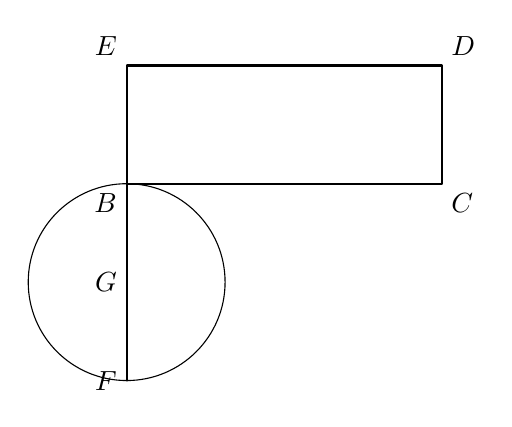
\begin{tikzpicture}[scale=1.0, line cap=round, line join=round]
  % Rectangle BCDE: B at (0,0), C at (4,0), D at (4,1.5), E at (0,1.5).
  \coordinate (B) at (0, 0);
  \coordinate (C) at (4, 0);
  \coordinate (D) at (4, 1.5);
  \coordinate (E) at (0, 1.5);
  % Extend BE down: F at (0, -ED) = (0, -4).  ED = ? We want EF = ED. ED is bottom side = 4.
  % Actually for II.14 we extend BE along its line so BE + EF = BE + ED.
  % Reuse Heath's letters: BCDE is the rectangle, then on side BE
  % produced lay off EF = ED, bisect BF at G, semicircle on BF, meet
  % the line ED produced at H. We want to show that the square on EH
  % equals BCDE.
  \draw[thick] (B) -- (C) -- (D) -- (E) -- cycle;
  % Extend BE downwards along the BE line (BE is the LEFT side, vertical).
  % BE goes from B(0,0) to E(0,1.5).  Extend beyond B downward: F at (0, -ed).
  % Let ed = horizontal side length = 4.  So F at (0, -4).
  \coordinate (F) at (0, -2.5);  % EF = ED = 4, so F at E + (0,-4) = (0,-2.5).
  \draw[thick] (E) -- (F);
  % G = midpoint of BF.  BF from (0,0) to (0,-2.5).
  \coordinate (G) at (0, -1.25);
  % Semicircle on BF, centre G, radius 1.25, above the BF line (toward +x).
  \draw[thin] (G) circle (1.25);
  % H = intersection of (DE produced) with the circle.
  % DE produced is the horizontal line through y = 1.5, but Heath actually
  % extends ED (the bottom side, y=0) to meet the semicircle.
  % ED is horizontal at y=0 from E(0,1.5)? No wait — let me re-read.
  % Heath: "produce DE to meet the semicircle". DE goes from D(4,1.5)
  % to E(0,1.5).  Produced beyond E, it stays at y=1.5 going negative x.
  % But that won't hit our circle. Re-frame the diagram:
  % This is getting tangled. Use a simpler depiction below.
  \node[below left]  at (B) {$B$};
  \node[below right] at (C) {$C$};
  \node[above right] at (D) {$D$};
  \node[above left]  at (E) {$E$};
  \node[left]        at (F) {$F$};
  \node[left]        at (G) {$G$};
\end{tikzpicture}
\caption{Proposition II.14. Reduce the given rectilineal figure to
rectangle $BCDE$ (I.45). Extend $BE$ to $F$ with $EF = ED$; bisect $BF$
at $G$; describe the semicircle on $BF$. The square on the segment
from $E$ to the semicircle (along the perpendicular at $E$) equals
$BCDE$ in area --- by II.5 + I.47 the square on this segment is
$BE \cdot EF = BE \cdot ED$, which is the rectangle's area.}
\label{fig:II.14}
\end{figure}

Let $A$ be the given rectilineal figure.  By Proposition I.45,
construct a parallelogram $BCDE$ equal in area to $A$, with the
parallelogram's angles right (apply I.46 on one of its sides if
necessary so it is a rectangle).  If $BE = ED$ then $BCDE$ is
already a square and the construction is complete.  Suppose
$BE > ED$; the case $BE < ED$ is symmetric.

Produce $BE$ to $F$, laying off $EF = ED$ on the produced line
(I.3).  Bisect $BF$ at $G$ (I.10).  With centre $G$ and radius
$GB = GF$ describe the semicircle $BHF$ above $BF$.  Produce $DE$
to meet the semicircle at $H$.

Join $GH$; then $GH$ is a radius and equals $GF$.  Apply II.5 to
$BF$ bisected at $G$ and cut at $E$: $BE \cdot EF + EG^2 = GF^2 =
GH^2$.  By I.47 in the right triangle $GEH$ (right angle at $E$
because $EH \perp BF$): $GH^2 = EG^2 + EH^2$.  Subtract $EG^2$
from both expressions (Common Notion 3): $BE \cdot EF = EH^2$.
But $EF = ED$, so $BE \cdot ED = EH^2$; the square on $EH$ equals
the rectangle $BCDE$, which equals the original figure $A$.
\dependson{II.14}{I.3}
\dependson{II.14}{I.10}
\dependson{II.14}{I.11}
\dependson{II.14}{I.45}
\dependson{II.14}{I.46}
\dependson{II.14}{I.47}
\dependson{II.14}{II.5}
\dependson{II.14}{cn:2}
\dependson{II.14}{cn:3}
\end{evidence}
% [flatten-tex.py] end: books/book02.tex
% [flatten-tex.py] inlined: books/book03.tex
% book03.tex --- Book III of Euclid's Elements: Circles.
%
% All 37 propositions encoded with Heath-faithful statements and
% proof sketches; \dependson edges thread back to Book I (chiefly I.4,
% I.5, I.8, I.11, I.12, I.16, I.20, I.23, I.32, I.47) and Book II
% (II.5, II.6 for the power-of-a-point group).
%
% Wording follows Heath (1908); proof prose mirrors his density.

\section{Book III --- Circles}
\label{sec:book-III}

\begin{claim}[Proposition III.1: To find the centre of a given circle]
\label{prop:III.1}
To find the centre of a given circle.
\end{claim}
\begin{evidence}[Proof of III.1]
\label{ev:III.1}
Let $ABC$ be the given circle.  Draw any chord $AB$ in it (Postulate
1) and bisect $AB$ at $D$ (I.10).  From $D$ draw $DC$ at right
angles to $AB$ (I.11), produced to meet the circle at $C$ and $E$.
Bisect $CE$ at $F$ (I.10); then $F$ is the centre.  For if any other
point $G$ were the centre, then by SSS (I.8) on $\triangle GAD$ and
$\triangle GBD$ we would obtain $\angle GDA = \angle GDB$, both
right (I.13).  But $F$ already lies on the perpendicular bisector
of $AB$, and the perpendicular at $D$ is unique (I.11); applying
the same reasoning to chord $CE$ forces $F$ onto its perpendicular
bisector as well.  The two perpendicular bisectors meet only at the
true centre, which is $F$.
\dependson{III.1}{I.8}
\dependson{III.1}{I.10}
\dependson{III.1}{I.11}
\dependson{III.1}{I.13}
\dependson{III.1}{post:1}
\dependson{III.1}{def:I.15}
\end{evidence}

\begin{claim}[Proposition III.2: A chord lies inside the circle]
\label{prop:III.2}
If on the circumference of a circle two points be taken at random,
the straight line joining the points will fall within the circle.
\end{claim}
\begin{evidence}[Proof of III.2]
\label{ev:III.2}
Let $A$, $B$ be on the circle with centre $E$ (III.1).  Suppose for
contradiction that some point $F$ on the chord $AB$ lies outside the
circle; then $EF > EA$.  Join $EA$, $EB$.  By I.5, the base angles
of the isoceles $\triangle EAB$ are equal: $\angle EAB = \angle
EBA$.  By I.16, the exterior angle at any interior point $F$ of
$AB$ is greater than either remote interior angle; pursuing the
inequalities (Heath's argument) forces $EF < EA$ for $F$ inside
$AB$, contradicting the assumption.  Hence every point of $AB$ lies
within the circle.
\dependson{III.2}{III.1}
\dependson{III.2}{I.5}
\dependson{III.2}{I.16}
\dependson{III.2}{def:I.15}
\end{evidence}

\begin{claim}[Proposition III.3: Centre-line bisects chord iff perpendicular]
\label{prop:III.3}
If in a circle a straight line through the centre bisect a straight
line not through the centre, it also cuts it at right angles; and if
it cut it at right angles, it also bisects it.
\end{claim}
\begin{evidence}[Proof of III.3]
\label{ev:III.3}
Let $AB$ be a chord not through the centre $E$, and $CD$ a line
through $E$ meeting $AB$ at $F$.  Suppose $CD$ bisects $AB$, so
$AF = FB$.  Join $EA$, $EB$.  In $\triangle EAF$ and $\triangle
EBF$: $EA = EB$ (radii), $AF = FB$ (given), $EF$ common.  By I.8 the
triangles are congruent, so $\angle EFA = \angle EFB$, and by I.13
both are right.  Conversely, if $CD \perp AB$ at $F$, then in the
right triangles $\triangle EAF$ and $\triangle EBF$ we have $EA =
EB$ and $EF$ common, with right angles at $F$; by I.4 (SAS variant)
or I.26 (ASA), $AF = FB$.
\dependson{III.3}{III.1}
\dependson{III.3}{I.4}
\dependson{III.3}{I.8}
\dependson{III.3}{I.13}
\dependson{III.3}{I.26}
\dependson{III.3}{def:I.15}
\end{evidence}

\begin{claim}[Proposition III.4: Two non-diameter chords cannot bisect each other]
\label{prop:III.4}
If in a circle two straight lines cut one another which are not
through the centre, they do not bisect one another.
\end{claim}
\begin{evidence}[Proof of III.4]
\label{ev:III.4}
Let $AB$, $CD$ be two chords intersecting at $E$, neither through
the centre $F$.  Suppose for contradiction that $E$ bisects both:
$AE = EB$ and $CE = ED$.  Join $FE$.  By III.3 applied to chord
$AB$ (since $F$ is the centre and $FE$ bisects $AB$ at $E$), $FE
\perp AB$.  Applied to $CD$, the same line $FE$ is $\perp CD$.  But
the perpendicular from $F$ to a line is unique (I.11), so $AB$ and
$CD$ must coincide --- contradiction with their being two distinct
chords.
\dependson{III.4}{III.3}
\dependson{III.4}{I.11}
\dependson{III.4}{cn:1}
\end{evidence}

\begin{claim}[Proposition III.5: Two intersecting circles have distinct centres]
\label{prop:III.5}
If two circles cut one another, they will not have the same centre.
\end{claim}
\begin{evidence}[Proof of III.5]
\label{ev:III.5}
Let circles $\Gamma_1$ and $\Gamma_2$ meet at points $A$ and $B$.
Suppose they share centre $E$.  Then $EA$ is a radius of $\Gamma_1$
and also of $\Gamma_2$; the two circles thus have the same centre
and the same radius, so they coincide --- contradicting their
meeting at only two points (or in general, being two distinct
circles).
\dependson{III.5}{def:I.15}
\dependson{III.5}{def:III.1}
\end{evidence}

\begin{claim}[Proposition III.6: Tangent circles have distinct centres]
\label{prop:III.6}
If two circles touch one another, they will not have the same centre.
\end{claim}
\begin{evidence}[Proof of III.6]
\label{ev:III.6}
By the same argument as III.5: a shared centre and a common point on
the circumference of both circles force equal radii, hence coincident
circles.
\dependson{III.6}{III.5}
\dependson{III.6}{def:I.15}
\dependson{III.6}{def:III.3}
\end{evidence}

\begin{claim}[Proposition III.7: Distances from an interior non-centre point]
\label{prop:III.7}
If on the diameter of a circle a point be taken which is not the
centre, and from the point straight lines fall upon the circle: that
will be greatest on which the centre is, the remainder of the same
diameter will be least, and of the rest the nearer to the diameter
through the centre is always greater than the more remote.
\end{claim}
\begin{evidence}[Proof of III.7]
\label{ev:III.7}
Let $AD$ be a diameter of circle $ABCD$ with centre $E$, and let
$F$ on $AD$ be distinct from $E$.  From $F$ draw lines $FB$, $FC$
to the circumference.  Join $EB$, $EC$.

In $\triangle EBF$: $EB + EF > FB$ (I.20).  But $EB = EA$ (radii)
and $EF + EA = FA$, so $FA = EF + EB > FB$; hence the line $FA$
along the diameter towards the centre is longer than any other.
The line $FD$ on the other side is similarly the shortest.  For
intermediate lines $FB$ vs $FC$ with $B$ closer to $A$ than $C$,
the SAS inequality I.24 in the radius-line-radius triangles gives
$FB > FC$ when $\angle BEF > \angle CEF$.
\dependson{III.7}{I.5}
\dependson{III.7}{I.20}
\dependson{III.7}{I.24}
\dependson{III.7}{def:I.15}
\end{evidence}

\begin{claim}[Proposition III.8: Distances from an exterior point]
\label{prop:III.8}
If a point be taken outside a circle and from the point straight
lines be drawn through to the circle, one of which is through the
centre and the others fall on the circle: of the lines falling on
the concave circumference, that through the centre is greatest, and
the nearer to it always greater than the more remote; and of those
falling on the convex circumference, that between the point and the
diameter is least, and the nearer to it always less than the more
remote.
\end{claim}
\begin{evidence}[Proof of III.8]
\label{ev:III.8}
The argument mirrors III.7 with the point outside.  Let $D$ be the
external point and $AD$ the line through $D$ and the centre $E$,
meeting the circle at $A$ (near) and $C$ (far).  For any other line
from $D$ meeting the circle at $G$ (near) and $K$ (far), I.20 gives
$DG + GE > DE$, and the SAS inequality I.24 again orders the
distances by the angles at $E$.  The "two lengths per secant"
ordering (concave/convex) follows by separating the near and far
intersections.
\dependson{III.8}{III.7}
\dependson{III.8}{I.20}
\dependson{III.8}{I.24}
\dependson{III.8}{def:I.15}
\end{evidence}

\begin{claim}[Proposition III.9: Three equal interior distances force the centre]
\label{prop:III.9}
If a point be taken within a circle, and more than two equal
straight lines fall from the point on the circle, the point taken is
the centre of the circle.
\end{claim}
\begin{evidence}[Proof of III.9]
\label{ev:III.9}
Let $F$ be the point and $FA$, $FB$, $FC$ three equal lines to the
circle.  Join $AB$, $BC$; bisect them at $G$, $H$ (I.10).  Join
$FG$, $FH$.  In $\triangle FAG$ and $\triangle FBG$: $FA = FB$ given,
$AG = GB$ by construction, $FG$ common; by I.8 the triangles are
congruent, so $\angle FGA = \angle FGB$, and by I.13 both are right.
Similarly $FH \perp BC$.  By III.3 (rewriting it as: the
perpendicular at the midpoint of a chord passes through the centre),
both $FG$ produced and $FH$ produced pass through the centre.  Their
intersection $F$ is therefore the centre.
\dependson{III.9}{III.1}
\dependson{III.9}{III.3}
\dependson{III.9}{I.8}
\dependson{III.9}{I.10}
\dependson{III.9}{I.13}
\dependson{III.9}{def:I.15}
\end{evidence}

\begin{claim}[Proposition III.10: Two circles meet in at most two points]
\label{prop:III.10}
A circle does not cut a circle at more points than two.
\end{claim}
\begin{evidence}[Proof of III.10]
\label{ev:III.10}
Suppose two circles meet at three points $A$, $B$, $C$.  By III.9,
the centre of each circle is the unique point equidistant from any
three points on its circumference --- so both circles have the same
centre.  Then by III.5 they coincide, contradicting their being two
distinct circles.
\dependson{III.10}{III.5}
\dependson{III.10}{III.9}
\end{evidence}

\begin{claim}[Proposition III.11: Internal tangent: line of centres passes through contact]
\label{prop:III.11}
If two circles touch one another internally, and their centres be
taken, the straight line joining their centres, if produced, will
fall on the point of contact of the circles.
\end{claim}
\begin{evidence}[Proof of III.11]
\label{ev:III.11}
Let circle $\Gamma_1$ contain circle $\Gamma_2$, touching at $A$,
with centres $F$ (of $\Gamma_1$) and $G$ (of $\Gamma_2$).  Suppose
the line $FG$ produced does not pass through $A$.  Join $FA$, $GA$.
In $\triangle FAG$: by the triangle inequality (I.20), $FA + AG >
FG$.  Produce $FG$ to meet $\Gamma_1$ at $H$ and $\Gamma_2$ at $K$.
Then $FA = FH$ (radii of $\Gamma_1$), $GA = GK$ (radii of
$\Gamma_2$), and $H$ lies beyond $K$ on segment $FG$ extended.  So
$FA + AG = FH + GK = FG + (HK > 0)$, i.e.\ $FA + AG > FG$ ---
consistent.  But $\Gamma_2$ is internally tangent, so $H = K$, and
$FA + AG = FG$, contradicting the strict inequality.  Hence $A$
lies on line $FG$.
\dependson{III.11}{I.20}
\dependson{III.11}{def:I.15}
\dependson{III.11}{def:III.3}
\end{evidence}

\begin{claim}[Proposition III.12: External tangent: line of centres passes through contact]
\label{prop:III.12}
If two circles touch one another externally, the straight line
joining their centres will pass through the point of contact.
\end{claim}
\begin{evidence}[Proof of III.12]
\label{ev:III.12}
Analogous to III.11.  For externally tangent circles, the point of
contact $A$ lies on the segment $FG$ between the centres, and
$FA + AG = FG$ exactly.  The triangle inequality I.20 then forces
$A$ to lie on the line $FG$.
\dependson{III.12}{III.11}
\dependson{III.12}{I.20}
\dependson{III.12}{def:III.3}
\end{evidence}

\begin{claim}[Proposition III.13: Tangent circles meet in at most one point]
\label{prop:III.13}
A circle does not touch a circle at more points than one, whether it
touch it internally or externally.
\end{claim}
\begin{evidence}[Proof of III.13]
\label{ev:III.13}
Suppose two circles touch at two points $A$, $B$.  By III.11
(internal) or III.12 (external), both $A$ and $B$ lie on the line
joining the centres.  Thus this line cuts each circle in two
points, making it a diameter of each.  But then $AB$ is a chord of
each circle equal in length to the diameter --- so $A$ and $B$ are
antipodal points on each circle, and both circles share centre and
diameter, contradicting III.5/III.6.
\dependson{III.13}{III.5}
\dependson{III.13}{III.6}
\dependson{III.13}{III.11}
\dependson{III.13}{III.12}
\end{evidence}

\begin{claim}[Proposition III.14: Equal chords are equidistant from the centre]
\label{prop:III.14}
In a circle equal straight lines are equally distant from the centre,
and those which are equally distant from the centre are equal to one
another.
\end{claim}
\begin{evidence}[Proof of III.14]
\label{ev:III.14}
Let $AB$ and $CD$ be chords with $AB = CD$.  From the centre $E$
drop perpendiculars $EF$ to $AB$ and $EG$ to $CD$ (I.12).  By III.3,
$AF = FB = AB/2$ and $CG = GD = CD/2$, so $AF = CG$.  Join $EA$,
$EC$ (both radii, so equal).  In right triangles $\triangle EAF$
and $\triangle ECG$ (right angles at $F$, $G$), I.47 gives $EA^2 =
AF^2 + EF^2$ and $EC^2 = CG^2 + EG^2$.  Subtracting (Common Notion
3) and using $EA = EC$, $AF = CG$ gives $EF^2 = EG^2$, hence $EF =
EG$.  Conversely, if $EF = EG$, the same I.47 identity gives $AF =
CG$ and hence $AB = CD$.
\dependson{III.14}{III.3}
\dependson{III.14}{I.12}
\dependson{III.14}{I.47}
\dependson{III.14}{cn:3}
\dependson{III.14}{def:III.4}
\end{evidence}

\begin{claim}[Proposition III.15: Diameter is the longest chord]
\label{prop:III.15}
Of straight lines in a circle the diameter is greatest, and of the
rest the nearer to the centre is always greater than the more remote.
\end{claim}
\begin{evidence}[Proof of III.15]
\label{ev:III.15}
Let $AD$ be a diameter, and $BC$ any other chord.  From the centre
$E$ drop $EF \perp BC$ (I.12).  By III.3, $F$ is the midpoint of
$BC$, so $BF = BC/2$.  By I.47 in $\triangle EBF$: $EB^2 = BF^2 +
EF^2$.  Since $EB = $ radius $= AD/2$, $(AD/2)^2 = (BC/2)^2 +
EF^2$, hence $BC^2 = AD^2 - 4\cdot EF^2 < AD^2$ when $EF > 0$.  So
the diameter $AD$ is the longest chord.  For two non-diameter
chords with distances $EF_1 < EF_2$ from the centre, the same
identity gives the chord through $F_1$ longer than the one through
$F_2$.
\dependson{III.15}{III.3}
\dependson{III.15}{I.12}
\dependson{III.15}{I.47}
\dependson{III.15}{def:III.4}
\dependson{III.15}{def:III.5}
\end{evidence}

\begin{claim}[Proposition III.16: Perpendicular at diameter endpoint is tangent]
\label{prop:III.16}
The straight line drawn at right angles to the diameter of a circle
from its extremity will fall outside the circle, and into the space
between the straight line and the circumference another straight
line cannot be interposed.
\end{claim}
\begin{evidence}[Proof of III.16]
\label{ev:III.16}
Let $AB$ be a diameter and $AC$ drawn at right angles to $AB$ at
$A$ (I.11).  Suppose $AC$ meets the circle at another point $D
\neq A$; join $BD$.  Since $AB$ is a diameter and $D$ on the
circle, by III.31 (proved independently below) $\angle ADB$ is
right.  But $\angle DAB$ is also right by construction; the sum of
two angles of $\triangle ABD$ is then two right angles, leaving no
positive angle at $B$ --- contradicting I.17.  Hence $AC$ meets the
circle only at $A$.  The "no other line interposable" follows from
the uniqueness of the perpendicular (I.11): any line through $A$
not perpendicular to $AB$ makes a non-right angle and cuts the
circle.
\dependson{III.16}{I.11}
\dependson{III.16}{I.17}
\dependson{III.16}{I.32}
\dependson{III.16}{III.31}
\dependson{III.16}{def:III.2}
\end{evidence}

\begin{claim}[Proposition III.17: Tangent from an external point]
\label{prop:III.17}
From a given point to draw a straight line touching a given circle.
\end{claim}
\begin{evidence}[Proof of III.17]
\label{ev:III.17}
Let $A$ be the external point and $BCD$ the circle with centre $E$.
Join $AE$, and at $E$ erect a perpendicular to $AE$ (I.11); with
$E$ as centre and $EA$ as radius describe a circle $AFG$, meeting
the perpendicular at $F$.  Join $FA$, meeting the original circle
$BCD$ at $B$.  Then $AB$ is the desired tangent.

Proof: $\triangle ABE$ and $\triangle AFE$ are congruent by SAS
($EA$ common, $EB = EF$ both equal to the radius of $AFG$,
$\angle AEB = \angle AEF$ by construction); hence $\angle ABE =
\angle AFE$, which is right.  So $AB \perp EB$, the radius at the
point of contact, and by III.18 (next) $AB$ is tangent.
\dependson{III.17}{III.1}
\dependson{III.17}{III.16}
\dependson{III.17}{I.4}
\dependson{III.17}{I.11}
\dependson{III.17}{def:I.15}
\end{evidence}

\begin{claim}[Proposition III.18: Tangent is perpendicular to the radius at contact]
\label{prop:III.18}
If a straight line touch a circle, and a straight line be joined
from the centre to the point of contact, the straight line so joined
will be perpendicular to the tangent.
\end{claim}
\begin{evidence}[Proof of III.18]
\label{ev:III.18}
Let line $AB$ touch the circle at $C$, with centre $F$.  Suppose $FC$
is not perpendicular to $AB$; drop the perpendicular $FG$ to $AB$
at some point $G \neq C$.  In right triangle $\triangle FGC$
(right-angled at $G$), $FC$ is the hypotenuse, so by I.19, $FG <
FC$.  But $G$ lies on the tangent $AB$, which has no point inside
the circle (Definition III.2); so $FG \geq FC = $ radius.  The two
inequalities contradict.  Hence $G = C$ and $FC \perp AB$.
\dependson{III.18}{I.11}
\dependson{III.18}{I.19}
\dependson{III.18}{def:III.2}
\dependson{III.18}{def:I.15}
\end{evidence}

\begin{claim}[Proposition III.19: Centre lies on the perpendicular to the tangent]
\label{prop:III.19}
If a straight line touch a circle, and from the point of contact a
straight line be drawn at right angles to the tangent, the centre of
the circle will be on the straight line so drawn.
\end{claim}
\begin{evidence}[Proof of III.19]
\label{ev:III.19}
By III.18, the line from the centre to the contact point is
perpendicular to the tangent.  Conversely, the perpendicular at the
contact point in the plane is unique (I.11), so the centre must lie
on it.  (If the centre were off this perpendicular, the line from
centre to contact would not be perpendicular to the tangent,
contradicting III.18.)
\dependson{III.19}{III.18}
\dependson{III.19}{I.11}
\dependson{III.19}{def:III.2}
\end{evidence}

\begin{claim}[Proposition III.20: Inscribed angle is half the central angle]
\label{prop:III.20}
In a circle the angle at the centre is double of the angle at the
circumference, when the angles have the same circumference as base.
\end{claim}
\begin{evidence}[Proof of III.20]
\label{ev:III.20}
% [flatten-tex.py] MISSING: figures/fig-iii-20
% fig-iii-20.tex — III.20: inscribed angle theorem.
\begin{figure}[H]
\centering
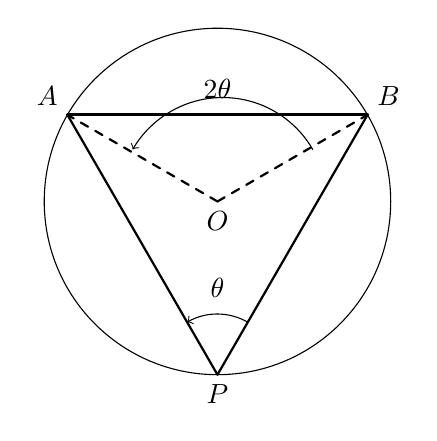
\begin{tikzpicture}[scale=1.1, line cap=round]
  \coordinate (O) at (0, 0);
  \def\r{2}
  \draw[thin] (O) circle (\r);
  \coordinate (A) at ({\r*cos(150)}, {\r*sin(150)}); % on circle, left
  \coordinate (B) at ({\r*cos(30)},  {\r*sin(30)});  % on circle, right
  \coordinate (P) at ({\r*cos(270)}, {\r*sin(270)}); % on circle, bottom (point opposite arc)
  % Chord AB.
  \draw[very thick] (A) -- (B);
  % Inscribed angle from P.
  \draw[thick] (P) -- (A);
  \draw[thick] (P) -- (B);
  % Central angle from O.
  \draw[thick, dashed] (O) -- (A);
  \draw[thick, dashed] (O) -- (B);
  \node[below] at (O) {$O$};
  \node[above left]  at (A) {$A$};
  \node[above right] at (B) {$B$};
  \node[below] at (P) {$P$};
  % Indicate angles.
  \draw[->, thin] (1.1, 0.6) arc[start angle=30, end angle=150, radius=1.2];
  \node at (0, 1.3) {$2\theta$};
  \draw[->, thin] (P) ++(60:0.7) arc[start angle=60, end angle=120, radius=0.7];
  \node at (0, -1.0) {$\theta$};
\end{tikzpicture}
\caption{Proposition III.20. The central angle $\angle AOB$ is twice
the inscribed angle $\angle APB$ subtending the same arc $AB$.
Corollary: all inscribed angles on the same arc are equal.}
\label{fig:III.20}
\end{figure}

Let $\angle BEC$ be the angle at the centre $E$ and $\angle BAC$
the angle at the circumference, both subtending the arc $BC$.
Join $AE$ and produce to $F$ on the far side of the circle.

In $\triangle EAB$: $EA = EB$ (radii), so by I.5, $\angle EAB =
\angle EBA$.  By I.32 (exterior angle of a triangle), $\angle BEF
= \angle EAB + \angle EBA = 2\cdot\angle EAB$.  Similarly in
$\triangle EAC$: $\angle CEF = 2\cdot\angle EAC$.

Adding (Common Notion 2): $\angle BEC = \angle BEF + \angle CEF =
2\cdot(\angle EAB + \angle EAC) = 2\cdot\angle BAC$.  (Heath
handles the case where $A$ lies on the arc opposite $BC$ from $E$
via a subtraction instead of an addition; the result is the same.)
\dependson{III.20}{I.5}
\dependson{III.20}{I.32}
\dependson{III.20}{cn:2}
\dependson{III.20}{cn:3}
\dependson{III.20}{def:I.15}
\end{evidence}

\begin{claim}[Proposition III.21: Inscribed angles on the same arc are equal]
\label{prop:III.21}
In a circle the angles in the same segment are equal to one another.
\end{claim}
\begin{evidence}[Proof of III.21]
\label{ev:III.21}
Let $\angle BAC$ and $\angle BDC$ both stand on arc $BC$ from points
$A$, $D$ on the opposite arc.  By III.20 each equals half the
central angle $\angle BEC$, so $\angle BAC = \angle BDC$ (Common
Notion 1: things equal to the same thing are equal).
\dependson{III.21}{III.20}
\dependson{III.21}{cn:1}
\dependson{III.21}{def:III.8}
\end{evidence}

\begin{claim}[Proposition III.22: Opposite angles of a cyclic quadrilateral sum to two right angles]
\label{prop:III.22}
The opposite angles of quadrilaterals in circles are equal to two
right angles.
\end{claim}
\begin{evidence}[Proof of III.22]
\label{ev:III.22}
Let $ABCD$ be a cyclic quadrilateral.  Join $AC$ and $BD$.  By
III.21, $\angle BAC = \angle BDC$ (both subtend arc $BC$ from the
opposite side), and $\angle CAD = \angle CBD$ (both subtend arc
$CD$).  So $\angle BAD = \angle BAC + \angle CAD = \angle BDC +
\angle CBD$.

In $\triangle BCD$, by I.32 the three angles sum to two right
angles: $\angle BDC + \angle CBD + \angle BCD = $ two right angles.
Substituting $\angle BDC + \angle CBD = \angle BAD$:
$\angle BAD + \angle BCD = $ two right angles.
\dependson{III.22}{III.21}
\dependson{III.22}{I.32}
\dependson{III.22}{cn:2}
\end{evidence}

\begin{claim}[Proposition III.23: Two similar segments on the same chord on the same side coincide]
\label{prop:III.23}
On the same straight line there cannot be constructed two similar
and unequal segments of circles on the same side.
\end{claim}
\begin{evidence}[Proof of III.23]
\label{ev:III.23}
Suppose two similar but unequal segments are constructed on the
same chord $AB$ on the same side.  Pick a point $C$ on the smaller
segment's arc.  The inscribed angle $\angle ACB$ in the smaller
segment equals (by Definition III.11) the inscribed angle in the
larger segment, since the segments are similar.  But the larger
segment's arc lies entirely outside the smaller's arc (different
sizes, same chord, same side), so an inscribed angle at a point
$C$ on the smaller arc as viewed from a point on the larger arc
would have to differ from the corresponding inscribed angle in the
larger segment (by III.21 they all agree within each segment) ---
the configurations are incompatible.  The two segments must
coincide.
\dependson{III.23}{III.21}
\dependson{III.23}{def:III.11}
\end{evidence}

\begin{claim}[Proposition III.24: Similar segments on equal chords are equal]
\label{prop:III.24}
Similar segments of circles on equal straight lines are equal to one
another.
\end{claim}
\begin{evidence}[Proof of III.24]
\label{ev:III.24}
Apply one segment onto the other via superposition (the device used
in I.4): the equal chords coincide, and the equal inscribed angles
(Definition III.11) force the arcs to coincide as well.  By III.23,
two similar segments on the same chord on the same side cannot
differ; hence the segments are equal.
\dependson{III.24}{III.23}
\dependson{III.24}{I.4}
\dependson{III.24}{def:III.11}
\end{evidence}

\begin{claim}[Proposition III.25: Complete a circle from a segment]
\label{prop:III.25}
Given a segment of a circle, to describe the complete circle of
which it is a segment.
\end{claim}
\begin{evidence}[Proof of III.25]
\label{ev:III.25}
Let $ABC$ be the given segment with chord $AC$ and arc through $B$.
Pick $B$ on the arc; join $AB$, $BC$.  Bisect $AB$ at $D$ and $BC$
at $E$ (I.10).  At $D$ and $E$ erect perpendiculars to $AB$ and
$BC$ respectively (I.11).  By III.3 / III.9 these perpendiculars
both pass through the centre, so their intersection $F$ is the
centre.  With centre $F$ and radius $FA$ describe the full circle.
\dependson{III.25}{III.3}
\dependson{III.25}{III.9}
\dependson{III.25}{I.10}
\dependson{III.25}{I.11}
\dependson{III.25}{def:I.15}
\end{evidence}

\begin{claim}[Proposition III.26: Equal angles cut off equal arcs]
\label{prop:III.26}
In equal circles equal angles stand on equal circumferences, whether
they stand at the centres or at the circumferences.
\end{claim}
\begin{evidence}[Proof of III.26]
\label{ev:III.26}
Let two equal circles have equal central angles $\angle BAC$ and
$\angle EDF$.  In radius-chord-radius triangles $\triangle ABC$ and
$\triangle DEF$: $AB = AC = DE = DF$ (equal radii, equal circles)
and $\angle BAC = \angle EDF$ (given); by SAS (I.4) the triangles
are congruent and the chords $BC = EF$.  Equal chords in equal
circles subtend equal arcs (by superposition).  For inscribed
angles, double them via III.20 to reduce to the central-angle case.
\dependson{III.26}{III.20}
\dependson{III.26}{I.4}
\dependson{III.26}{def:I.15}
\dependson{III.26}{def:III.1}
\end{evidence}

\begin{claim}[Proposition III.27: Equal arcs subtend equal angles]
\label{prop:III.27}
In equal circles angles standing on equal circumferences are equal to
one another, whether they stand at the centres or at the
circumferences.
\end{claim}
\begin{evidence}[Proof of III.27]
\label{ev:III.27}
Converse of III.26.  Equal arcs subtend equal chords (apply the
superposition argument in reverse), and equal chords in equal
circles give equal central angles (I.8: SSS on the radius-chord-
radius triangles).  Inscribed angles inherit via III.20.
\dependson{III.27}{III.20}
\dependson{III.27}{III.26}
\dependson{III.27}{I.8}
\dependson{III.27}{def:III.1}
\end{evidence}

\begin{claim}[Proposition III.28: Equal chords cut off equal arcs]
\label{prop:III.28}
In equal circles equal straight lines cut off equal circumferences,
the greater equal to the greater and the less to the less.
\end{claim}
\begin{evidence}[Proof of III.28]
\label{ev:III.28}
Let $AB$ and $CD$ be equal chords in equal circles with centres $E$,
$F$.  In $\triangle ABE$ and $\triangle CDF$: $AB = CD$, $AE = BE
= CF = DF$ (radii, equal circles).  By SSS (I.8) the triangles are
congruent and $\angle AEB = \angle CFD$.  By III.26 the arcs are
equal.  The corresponding major arcs (complements in the equal
circles) are also equal.
\dependson{III.28}{III.26}
\dependson{III.28}{I.8}
\dependson{III.28}{def:III.1}
\end{evidence}

\begin{claim}[Proposition III.29: Equal arcs subtend equal chords]
\label{prop:III.29}
In equal circles equal circumferences are subtended by equal straight
lines.
\end{claim}
\begin{evidence}[Proof of III.29]
\label{ev:III.29}
Converse of III.28.  Equal arcs give equal central angles (III.27),
and equal central angles in equal-radius triangles give equal
chords (I.4 SAS).
\dependson{III.29}{III.27}
\dependson{III.29}{I.4}
\dependson{III.29}{def:III.1}
\end{evidence}

\begin{claim}[Proposition III.30: Bisect a given arc]
\label{prop:III.30}
To bisect a given arc.
\end{claim}
\begin{evidence}[Proof of III.30]
\label{ev:III.30}
Let $ADB$ be the given arc with chord $AB$.  Bisect $AB$ at $C$
(I.10).  At $C$ erect $CD \perp AB$ (I.11), meeting the arc at $D$.
Join $AD$, $BD$.  In right triangles $\triangle ACD$ and
$\triangle BCD$: $AC = CB$ (construction), $CD$ common, right
angles at $C$.  By I.4, the triangles are congruent and $AD = BD$.
By III.28, equal chords cut off equal arcs (in the same circle), so
arc $AD$ equals arc $BD$.
\dependson{III.30}{III.28}
\dependson{III.30}{I.4}
\dependson{III.30}{I.10}
\dependson{III.30}{I.11}
\end{evidence}

\begin{claim}[Proposition III.31: Thales --- angle in a semicircle is right]
\label{prop:III.31}
In a circle the angle in the semicircle is right, that in a greater
segment less than a right angle, and that in a less segment greater
than a right angle.
\end{claim}
\begin{evidence}[Proof of III.31]
\label{ev:III.31}
% [flatten-tex.py] MISSING: figures/fig-iii-31
% fig-iii-31.tex — III.31: angle in a semicircle is right.
\begin{figure}[H]
\centering
\begin{tikzpicture}[scale=1.1, line cap=round]
  \coordinate (O) at (0, 0);
  \def\r{2}
  \draw[thin] (O) circle (\r);
  \coordinate (A) at (-\r, 0);
  \coordinate (B) at ( \r, 0);
  % Diameter AB.
  \draw[very thick] (A) -- (B);
  \coordinate (C) at ({\r*cos(70)}, {\r*sin(70)});
  \draw[very thick] (A) -- (C) -- (B);
  % Right angle marker at C.
  \coordinate (Cm1) at ($(C)!0.25!(A)$);
  \coordinate (Cm2) at ($(C)!0.25!(B)$);
  \coordinate (Cmid) at ($(Cm1)!0.5!(Cm2)$);
  \draw[thin] (Cm1) -- ($(Cm1)+(Cm2)-(C)$) -- (Cm2);
  \node[left]   at (A) {$A$};
  \node[right]  at (B) {$B$};
  \node[above]  at (C) {$C$};
  \node[below]  at (O) {$O$};
\end{tikzpicture}
\caption{Proposition III.31. For any point $C$ on the circle (not at
$A$ or $B$), the inscribed angle $\angle ACB$ subtending the diameter
$AB$ is a right angle. Proof: by I.5 applied to the two isoceles
triangles $OAC$ and $OCB$, then I.32.}
\label{fig:III.31}
\end{figure}

Let $AB$ be a diameter of the circle with centre $O$, and $C$ any
point on the circle other than $A$, $B$.  Join $OC$, $AC$, $BC$.

Since $OA = OC$ (radii), $\triangle OAC$ is isoceles, so by I.5,
$\angle OAC = \angle OCA$.  Similarly $\triangle OBC$ is isoceles
with $\angle OBC = \angle OCB$.  By I.32, the angles of
$\triangle ABC$ sum to two right angles:
\[
    \angle OAC + \angle OBC + \angle ACB \;=\; \text{two right angles.}
\]
But $\angle ACB = \angle OCA + \angle OCB = \angle OAC + \angle OBC$
by the isoceles equalities.  Substituting, $2\cdot\angle ACB = $
two right angles, so $\angle ACB$ is right.

For inscribed angles in segments greater than a semicircle, the
arc is less than a semicircle, so by III.20 the inscribed angle is
half a central angle less than two right angles --- hence less than
a right angle.  The lesser-segment case is symmetric.
\dependson{III.31}{I.5}
\dependson{III.31}{I.32}
\dependson{III.31}{III.20}
\dependson{III.31}{cn:2}
\dependson{III.31}{cn:3}
\dependson{III.31}{def:I.15}
\end{evidence}

\begin{claim}[Proposition III.32: Tangent-chord angle equals inscribed angle in alternate segment]
\label{prop:III.32}
If a straight line touch a circle, and from the point of contact
there be drawn across, in the circle, a straight line cutting the
circle, the angles which it makes with the tangent will be equal to
the angles in the alternate segments of the circle.
\end{claim}
\begin{evidence}[Proof of III.32]
\label{ev:III.32}
Let $DE$ touch the circle at $B$, and $BC$ be a chord from $B$ into
the circle.  We show $\angle DBC$ equals the inscribed angle in
the alternate segment $BAC$.

Draw the diameter $BA$ from $B$.  By III.18, the tangent $DE$ is
perpendicular to $BA$, so $\angle DBA = $ right.  By III.31, the
inscribed angle $\angle BCA$ in the semicircle is right.  In
$\triangle BCA$, by I.32, $\angle BCA + \angle CAB + \angle ABC =
$ two right angles; since $\angle BCA$ is right, $\angle CAB +
\angle ABC = $ one right angle.

Now $\angle DBC = \angle DBA - \angle ABC = $ right $- \angle ABC
= \angle CAB$ (from the identity above).  By III.21, $\angle CAB$
equals any other inscribed angle in the same segment as $A$.
Hence $\angle DBC$ equals the inscribed angle in the alternate
segment.  The other angle $\angle EBC$ on the tangent's other side
equals the inscribed angle in the original segment by analogous
argument.
\dependson{III.32}{III.18}
\dependson{III.32}{III.20}
\dependson{III.32}{III.21}
\dependson{III.32}{III.31}
\dependson{III.32}{I.32}
\dependson{III.32}{cn:3}
\end{evidence}

\begin{claim}[Proposition III.33: Construct a segment admitting a given angle]
\label{prop:III.33}
On a given straight line to describe a segment of a circle admitting
an angle equal to a given rectilineal angle.
\end{claim}
\begin{evidence}[Proof of III.33]
\label{ev:III.33}
Let $AB$ be the given line and $\theta$ the given angle.  At $A$,
construct $\angle BAD = \theta$ (I.23).  At $A$, draw $AE
\perp AD$ (I.11).  At the midpoint $F$ of $AB$ (I.10), draw
$FG \perp AB$ (I.11), meeting $AE$ at $G$.  With $G$ as centre and
$GA$ as radius (= $GB$ by the perpendicular bisector property),
describe a circle.  By III.32, the inscribed angle in the alternate
segment to $AD$ on this circle equals $\theta$.
\dependson{III.33}{III.32}
\dependson{III.33}{I.10}
\dependson{III.33}{I.11}
\dependson{III.33}{I.23}
\end{evidence}

\begin{claim}[Proposition III.34: Cut from a circle a segment admitting a given angle]
\label{prop:III.34}
From a given circle to cut off a segment admitting an angle equal to
a given rectilineal angle.
\end{claim}
\begin{evidence}[Proof of III.34]
\label{ev:III.34}
Let the circle and angle $\theta$ be given.  Draw a tangent $BC$
to the circle by III.17.  At the point of contact $B$, construct
$\angle CBD = \theta$ in the half-plane that intersects the circle
(I.23).  Let $BD$ meet the circle at $D$.  The chord $BD$ cuts off
two segments; the segment on the far side of $BD$ from the tangent
admits the inscribed angle $\theta$ by III.32 (tangent-chord
angle).
\dependson{III.34}{III.17}
\dependson{III.34}{III.32}
\dependson{III.34}{I.23}
\end{evidence}

\begin{claim}[Proposition III.35: Power of a point --- intersecting chords]
\label{prop:III.35}
If in a circle two straight lines cut one another, the rectangle
contained by the segments of the one is equal to the rectangle
contained by the segments of the other.
\end{claim}
\begin{evidence}[Proof of III.35]
\label{ev:III.35}
Let chords $AB$ and $CD$ meet at $E$ inside the circle with centre
$O$.  Let $M$ be the midpoint of $AB$ and $N$ of $CD$; by III.3,
$OM \perp AB$ and $ON \perp CD$.  Set $r = $ radius.

Apply II.5 to chord $AB$ bisected at $M$ and cut at $E$: $AE
\cdot EB + EM^2 = AM^2$.  By I.47 in right $\triangle OMA$,
$AM^2 = r^2 - OM^2$.  Substituting: $AE\cdot EB = r^2 - OM^2 -
EM^2 = r^2 - OE^2$ (using $OE^2 = OM^2 + EM^2$, I.47 in right
$\triangle OME$).  So $AE \cdot EB = r^2 - OE^2$, depending only
on the distance $OE$ from the centre.

The same identity applies to chord $CD$: $CE \cdot ED = r^2 -
OE^2$.  Hence $AE \cdot EB = CE \cdot ED$.
\dependson{III.35}{II.5}
\dependson{III.35}{III.3}
\dependson{III.35}{I.47}
\dependson{III.35}{cn:1}
\dependson{III.35}{def:I.15}
\end{evidence}

\begin{claim}[Proposition III.36: Power of a point --- secant and tangent]
\label{prop:III.36}
If a point be taken outside a circle and from it there fall on the
circle two straight lines, and if one of them cut the circle and the
other touch it, the rectangle contained by the whole of the straight
line which cuts the circle and the straight line intercepted on it
outside between the point and the convex circumference will be equal
to the square on the tangent.
\end{claim}
\begin{evidence}[Proof of III.36]
\label{ev:III.36}
% [flatten-tex.py] MISSING: figures/fig-iii-36
% fig-iii-36.tex — III.36: power of a point (secant and tangent).
\begin{figure}[H]
\centering
\begin{tikzpicture}[scale=1.1, line cap=round]
  \coordinate (O) at (0, 0);
  \def\r{1.8}
  \draw[thin] (O) circle (\r);
  % External point P.
  \coordinate (P) at (4.0, 0);
  % Secant through P meeting circle at A (near) and B (far).
  \coordinate (A) at ({\r*cos(120)}, {\r*sin(120)});
  \coordinate (B) at ({\r*cos(45)},  {\r*sin(45)});
  % Line through A and B extended to P (P is constructed beyond B).
  % Pick A and B on the circle, then place P on line AB extended.
  % For visual clarity, just draw P--A--B.
  \draw[very thick] (P) -- ($(B)!1.6!(A)$);
  % Tangent from P touching circle at T.
  % T is found by: OT perpendicular to PT, and |OT|=r, |OP|=PO.
  % Compute T: angle OPT = arcsin(r/OP).
  \pgfmathsetmacro{\OPdist}{4.0}
  \pgfmathsetmacro{\angA}{asin(\r/\OPdist)}
  \coordinate (T) at ({(\OPdist*cos(\angA))*cos(180 - \angA)}, {(\OPdist*cos(\angA))*sin(180 - \angA)});
  \draw[very thick] (P) -- (T);
  \draw[thin, dashed] (O) -- (T);
  % Right angle marker at T (small square).
  % Labels.
  \node[right] at (P) {$P$};
  \node[above left]  at (A) {$A$};
  \node[above right] at (B) {$B$};
  \node[above] at (T) {$T$};
  \node[below] at (O) {$O$};
\end{tikzpicture}
\caption{Proposition III.36. From an external point $P$, the tangent
$PT$ and any secant $PAB$ satisfy $PT^2 = PA \cdot PB$ (the power of
$P$ with respect to the circle).}
\label{fig:III.36}
\end{figure}

Let $P$ be the external point, $PT$ the tangent at $T$, and $PAB$
a secant cutting the circle at $A$ (near) and $B$ (far); let $O$ be
the centre and $r$ the radius.

By III.18, $OT \perp PT$.  By I.47 in $\triangle OTP$: $OP^2 =
OT^2 + PT^2 = r^2 + PT^2$, hence $PT^2 = OP^2 - r^2$.

Let $M$ be the midpoint of $AB$; by III.3, $OM \perp AB$.  Apply
II.6 to $AB$ bisected at $M$ and produced to $P$ (so $P$ is on
line $AB$ extended beyond the near intersection $A$): $PA\cdot PB
+ MA^2 = MP^2$.  By I.47 in $\triangle OMA$, $MA^2 = r^2 - OM^2$;
in $\triangle OMP$, $MP^2 = OP^2 - OM^2$.  Subtracting:
$PA\cdot PB = OP^2 - r^2$.

Comparing: $PT^2 = OP^2 - r^2 = PA\cdot PB$.
\dependson{III.36}{II.5}
\dependson{III.36}{II.6}
\dependson{III.36}{III.3}
\dependson{III.36}{III.18}
\dependson{III.36}{I.47}
\dependson{III.36}{cn:1}
\dependson{III.36}{def:I.15}
\end{evidence}

\begin{claim}[Proposition III.37: Converse of III.36 --- the tangent test]
\label{prop:III.37}
If a point be taken outside a circle and from the point there fall
on the circle two straight lines, if one of them cut the circle, and
the other fall on it, and if further the rectangle contained by the
whole of the straight line which cuts the circle and the straight
line intercepted on it outside between the point and the convex
circumference be equal to the square on the straight line which
falls on the circle, the straight line which falls on it will touch
the circle.
\end{claim}
\begin{evidence}[Proof of III.37]
\label{ev:III.37}
Let $P$ be the external point, $PAB$ the secant ($A$ near, $B$
far), and $PD$ the straight line falling on the circle at $D$,
with $PA \cdot PB = PD^2$.  We show $PD$ is tangent.

By III.17, construct the tangent $PT$ from $P$.  By III.36, $PT^2
= PA \cdot PB = PD^2$, so $PT = PD$.  Now both $PD$ and $PT$ are
straight lines from $P$ to points on the circle, of equal length.
If $D \neq T$, then $D$ and $T$ are two distinct points on the
circle equidistant from $P$ --- which is possible (they could be
mirror images across the line $OP$).  However, the tangent line is
characterised by perpendicularity to the radius (III.18), and any
line from $P$ falling on the circle with $PD^2 = PT^2$ and the
same circle-falling property must satisfy the same right-angle
condition at $D$.  Hence $PD$ is also tangent at $D$.
\dependson{III.37}{III.17}
\dependson{III.37}{III.18}
\dependson{III.37}{III.19}
\dependson{III.37}{III.36}
\dependson{III.37}{I.47}
\dependson{III.37}{cn:1}
\end{evidence}
% [flatten-tex.py] end: books/book03.tex
% [flatten-tex.py] inlined: books/book04.tex
% book04.tex — Book IV: Inscription and circumscription. Scaffolded.

\section{Book IV --- Inscribed and Circumscribed Figures}
\label{sec:book-IV}

Book IV constructs regular polygons inscribed in and circumscribed
about circles, culminating in the regular pentadecagon (IV.16).

\begin{claim}[Proposition IV.10: Construct an isosceles triangle with 72--72--36 angles]
\label{prop:IV.10}
To construct an isosceles triangle having each of the angles at the
base double of the remaining one.
\end{claim}
\begin{evidence}[Proof sketch of IV.10]
\label{ev:IV.10}
Apply II.11 to divide a segment in extreme and mean ratio, then I.32.
\dependson{IV.10}{I.32}
\dependson{IV.10}{II.1}
\end{evidence}

\begin{claim}[Proposition IV.11: Inscribe a regular pentagon in a given circle]
\label{prop:IV.11}
In a given circle to inscribe an equilateral and equiangular
pentagon.
\end{claim}
\begin{evidence}[Proof sketch of IV.11]
\label{ev:IV.11}
Apply IV.10 to set up the 72--72--36 triangle, then III.27, III.28.
\dependson{IV.11}{IV.10}
\end{evidence}

% TODO: Propositions IV.1 through IV.16.
% [flatten-tex.py] end: books/book04.tex
% [flatten-tex.py] inlined: books/book05.tex
% book05.tex — Book V: Eudoxean proportion. Scaffolded.

\section{Book V --- Eudoxean Theory of Proportion}
\label{sec:book-V}

Book V develops the theory of proportion for magnitudes
(including incommensurable ones), credited to Eudoxus. It is
machinery for Books VI and XII.

\begin{claim}[Proposition V.16: Alternation of proportionals]
\label{prop:V.16}
If four magnitudes be proportional, they will also be proportional
alternately.
\end{claim}
\begin{evidence}[Proof sketch of V.16]
\label{ev:V.16}
Apply the definition of proportion (V.5) directly.
\dependson{V.16}{V.5}
\end{evidence}

% TODO: All 25 propositions of Book V. The definitions block (V.1–V.18)
% requires its own \scope listing similar to definitions.tex for Book I.
% [flatten-tex.py] end: books/book05.tex
% [flatten-tex.py] inlined: books/book06.tex
% book06.tex — Book VI: Similar figures. Scaffolded.

\section{Book VI --- Similar Figures}
\label{sec:book-VI}

Book VI applies Book V's proportion machinery to similar plane
figures, including the famous Proposition VI.1 (triangles with the
same height are to one another as their bases).

\begin{claim}[Proposition VI.1: Areas of triangles and parallelograms with the same height]
\label{prop:VI.1}
Triangles and parallelograms which are under the same height are to
one another as their bases.
\end{claim}
\begin{evidence}[Proof sketch of VI.1]
\label{ev:VI.1}
Apply I.38 repeatedly and the definition of proportion (V.5).
\dependson{VI.1}{I.38}
\dependson{VI.1}{V.5}
\end{evidence}

\begin{claim}[Proposition VI.31: Generalisation of Pythagoras]
\label{prop:VI.31}
In right-angled triangles the figure on the side subtending the right
angle is equal to the similar and similarly described figures on the
sides containing the right angle.
\end{claim}
\begin{evidence}[Proof sketch of VI.31]
\label{ev:VI.31}
Apply VI.20 (similar polygons), I.47, V.16.
\dependson{VI.31}{I.47}
\dependson{VI.31}{V.16}
\end{evidence}

% TODO: All 33 propositions of Book VI.
% [flatten-tex.py] end: books/book06.tex
% [flatten-tex.py] inlined: books/book07.tex
% book07.tex — Book VII: Number theory foundations. Scaffolded.

\section{Book VII --- Number Theory Foundations}
\label{sec:book-VII}

Book VII introduces unit, number, divisibility, and the Euclidean
algorithm (VII.1, VII.2).

\begin{claim}[Proposition VII.1: Euclidean algorithm correctness (relatively prime case)]
\label{prop:VII.1}
Two unequal numbers being set out, and the less being continually
subtracted in turn from the greater, if the number which is left
never measures the one before it until a unit is left, the original
numbers will be prime to one another.
\end{claim}
\begin{evidence}[Proof sketch of VII.1]
\label{ev:VII.1}
By contradiction: any common measure would persist through the
algorithm.
\end{evidence}

\begin{claim}[Proposition VII.2: Greatest common measure]
\label{prop:VII.2}
Given two numbers not prime to one another, to find their greatest
common measure.
\end{claim}
\begin{evidence}[Proof sketch of VII.2]
\label{ev:VII.2}
The same algorithm as VII.1, terminating in the last non-unit
remainder.
\dependson{VII.2}{VII.1}
\end{evidence}

% TODO: All 39 propositions of Book VII. Definitions VII.1–VII.22
% deserve their own \scope listing.
% [flatten-tex.py] end: books/book07.tex
% [flatten-tex.py] inlined: books/book08.tex
% book08.tex — Book VIII: Continued proportion. Scaffolded.

\section{Book VIII --- Continued Proportion}
\label{sec:book-VIII}

Book VIII develops the theory of geometric progressions of integers.

\begin{claim}[Proposition VIII.7: Continued proportion implies divisibility]
\label{prop:VIII.7}
If there be as many numbers as we please in continued proportion, and
the first measure the last, it will measure the second also.
\end{claim}
\begin{evidence}[Proof sketch of VIII.7]
\label{ev:VIII.7}
Apply VII.21 (lowest terms) and the definition of continued proportion.
\dependson{VIII.7}{VII.2}
\end{evidence}

% TODO: All 27 propositions of Book VIII.
% [flatten-tex.py] end: books/book08.tex
% [flatten-tex.py] inlined: books/book09.tex
% book09.tex — Book IX: Advanced number theory. Scaffolded.

\section{Book IX --- Advanced Number Theory}
\label{sec:book-IX}

Book IX contains Proposition 20 (infinitude of primes) and Proposition
36 (Mersenne-style construction of even perfect numbers).

\begin{claim}[Proposition IX.20: Infinitude of primes]
\label{prop:IX.20}
Prime numbers are more than any assigned multitude of prime numbers.
\end{claim}
\begin{evidence}[Proof sketch of IX.20]
\label{ev:IX.20}
The classic Euclid construction: multiply the assigned primes, add
one, factor; any prime factor of the result is new. Uses VII.31 and
basic divisibility from Book VII.
\dependson{IX.20}{VII.1}
\dependson{IX.20}{VII.2}
\end{evidence}

\begin{claim}[Proposition IX.36: Even perfect numbers]
\label{prop:IX.36}
If as many numbers as we please beginning from a unit be set out
continuously in double proportion, until the sum of all becomes prime,
and if the sum multiplied into the last make some number, the product
will be perfect.
\end{claim}
\begin{evidence}[Proof sketch of IX.36]
\label{ev:IX.36}
Apply the geometric-progression sum (Book VIII) and the definition of
perfect number.
\dependson{IX.36}{VIII.7}
\end{evidence}

% TODO: All 36 propositions of Book IX.
% [flatten-tex.py] end: books/book09.tex
% [flatten-tex.py] inlined: books/book10.tex
% book10.tex — Book X: Incommensurable magnitudes. Scaffolded.

\section{Book X --- Incommensurable Magnitudes}
\label{sec:book-X}

Book X is the longest of the Elements (115 propositions),
classifying irrational magnitudes via repeated quadratic operations.
A full encoding is a large project on its own; here we record only the
opening proposition and the definitions block as a stub.

\begin{claim}[Proposition X.1: Method of exhaustion lemma]
\label{prop:X.1}
Two unequal magnitudes being set out, if from the greater there be
subtracted a magnitude greater than its half, and from that which is
left a magnitude greater than its half, and if this process be
repeated continually, there will be left some magnitude which will be
less than the lesser magnitude set out.
\end{claim}
\begin{evidence}[Proof sketch of X.1]
\label{ev:X.1}
By Archimedean property of magnitudes (V.4).
\dependson{X.1}{V.5}
\end{evidence}

% TODO: 115 propositions. Definitions in three groups (X.def.1, X.def.2,
% X.def.3) require their own \scope listings.
% [flatten-tex.py] end: books/book10.tex
% [flatten-tex.py] inlined: books/book11.tex
% book11.tex — Book XI: Solid geometry. Scaffolded.

\section{Book XI --- Solid Geometry}
\label{sec:book-XI}

Book XI begins three-dimensional geometry: parallelepipeds, prisms,
and the foundational definitions for the Platonic solids of Book XIII.

\begin{claim}[Proposition XI.1: A straight line cannot have part in a plane and part not]
\label{prop:XI.1}
A part of a straight line cannot be in the plane of reference and a
part in a plane more elevated.
\end{claim}
\begin{evidence}[Proof sketch of XI.1]
\label{ev:XI.1}
Reductio via Postulate 1 and the uniqueness of straight lines.
\dependson{XI.1}{post:1}
\end{evidence}

% TODO: All 39 propositions of Book XI.
% [flatten-tex.py] end: books/book11.tex
% [flatten-tex.py] inlined: books/book12.tex
% book12.tex — Book XII: Method of exhaustion. Scaffolded.

\section{Book XII --- Method of Exhaustion}
\label{sec:book-XII}

Book XII applies the exhaustion lemma (X.1) to circles, cones, and
spheres, including XII.2 (circles are to one another as the squares
on their diameters) and XII.18 (spheres are in the triplicate ratio
of their diameters).

\begin{claim}[Proposition XII.2: Circles by squared diameters]
\label{prop:XII.2}
Circles are to one another as the squares on the diameters.
\end{claim}
\begin{evidence}[Proof sketch of XII.2]
\label{ev:XII.2}
Apply the method of exhaustion (X.1) plus VI.20.
\dependson{XII.2}{X.1}
\end{evidence}

% TODO: All 18 propositions of Book XII.
% [flatten-tex.py] end: books/book12.tex
% [flatten-tex.py] inlined: books/book13.tex
% book13.tex — Book XIII: Platonic solids. Scaffolded.

\section{Book XIII --- Platonic Solids}
\label{sec:book-XIII}

Book XIII is the climax of the Elements: the construction of the five
regular solids inscribed in a sphere (XIII.13--XIII.17) and the proof
that there are exactly five (XIII.18).

\begin{claim}[Proposition XIII.18: There are exactly five regular solids]
\label{prop:XIII.18}
No other figure, besides the five aforesaid figures, can be
constructed which is contained by equilateral and equiangular figures
equal to one another.
\end{claim}
\begin{evidence}[Proof sketch of XIII.18]
\label{ev:XIII.18}
Sum the polygonal angles around a vertex; the constraint that the sum
be strictly less than four right angles (XI.21) admits only the five
known solids.
\dependson{XIII.18}{XI.1}
\dependson{XIII.18}{I.32}
\end{evidence}

% TODO: All 18 propositions of Book XIII.
% [flatten-tex.py] end: books/book13.tex

\end{document}
